% !TEX root = TI5.tex

\section{Equivalence of tensor isomorphism problems}

\subsection{A review of two gadgets for partition tensor isomorphism}


A key problem in the development of the complexity class $\cc{TI}$ is to reduce \emph{partitioned} tensor isomorphism reduces to ordinary \TI \cite{FGS19}. Two gadgets have been developed to achieve the reduction, the first one in \cite{FGS19}, and the second one in \cite{TI4}. 

To use these gadgets for commutative rings instead of fields, some issues arise, and as a result, we need to combine ideas from both gadget designs. 

In this subsection, we shall review the partitioned tensor isomorphism problem, review the two gadgets, demonstrate some issues for using them in commutative rings, and then explain on how to overcome them.

\paragraph{The partitioned tensor isomorphism problem.} Briefly speaking, the partitioned tensor isomorphism problem asks for isomorphisms between tensors whose indices in one or more directions are partitioned into blocks that must be preserved. 

\begin{definition}\label{def:pTI}
	Given $\tA, \tB\in \T(n\times m\times \ell, \F)$, and a partition of $[\ell]=D_1\cup D_2\cup \dots \cup D_L$, the \algprobm{Partitioned Tensor Isomorphism} (\pTI) problem asks whether there exists $(P, Q, R)$ that sends $\tA$ to $\tB$, where $P\in \GL(n, \F)$, $Q\in\GL(m, \F)$, and $R\in\GL(\ell_1, \F)\times\dots\times\GL(\ell_L, \F)$ viewed as a subgroup of block-diagonal matrices in $\GL(\ell, \F)$ respecting the partition.
\end{definition}
One can of course consider partitions in all three directions, but for clarity of exposition we focus just on one direction in this section. This problem can be viewed as the tensor analogue of the classical \emph{colored} graph isomorphism problem \cite{KST93}; see \cite{TI4} for a discussion.

%In \cite{FGS19}, they show that many tensor problems reduce to \algprobm{Partitioned Tensor Isomorphism}, and that the latter reduces to ordinary \TI, albeit with quadratic length increase.


\subsubsection{The Futorny--Grochow--Sergeichuk (FGS) gadget}\label{sec:FGS}

The first reduction from \pTI to \TI was done using a gadget designed in \cite{FGS19}, which we call the \emph{Futorny--Grochow--Sergeichuk gadget}, or FGS gadget for short. This gadget can be naturally viewed as corresponding to the star graph gadget, see e.g. the discussion in \cite[Sec.~3]{TI2}.
%, which we now explain (see also the discussion in \cite[Sec.~3]{GQ2}).

\begin{example}[An example of the FGS gadget]\label{ex:FGS}
To see how the FGS gadget works, consider the following example. By slicing along the third index, a $3$-way array $\tA\in\T(n\times m\times 6, \F)$ can be represented as a tuple of six matrices $\vA=(A_1, \dots, A_6)$. Suppose $\ell=6$ and $L=3$, $n\leq m$, with $[6]$ partitioned into $\{1, 2\}, \{3, 4\}, \{5, 6\}$. 

To reduce this \pTI instance to \TI following \cite{FGS19}, we construct 
\[\tilde A_1=\begin{bmatrix}
	A_1 & 0 & 0 & 0 & 0 & 0 & 0 \\
	0 & \idmat_{n+1} & 0 & 0 & 0 & 0 & 0 \\
	0 & 0 & 0 & 0 & 0 & 0 & 0 \\
	0 & 0 & 0 & 0 & 0 & 0 & 0 \\
\end{bmatrix}, 
\tilde A_2=\begin{bmatrix}
	A_ 2& 0 & 0 & 0 & 0 & 0 & 0 \\
	0 & 0 & \idmat_{n+1} & 0 & 0 & 0 & 0 \\
	0 & 0 & 0 & 0 & 0 & 0 & 0 \\
	0 & 0 & 0 & 0 & 0 & 0 & 0 \\
\end{bmatrix},\]
\[
\tilde A_3=\begin{bmatrix}
	A_3 & 0 & 0 & 0 & 0 & 0 & 0 \\
	0 & 0 & 0 & 0 & 0 & 0 & 0 \\
	0 & 0 & 0 & \idmat_{2n+2} & 0 & 0 & 0 \\
	0 & 0 & 0 & 0 & 0 & 0 & 0 \\
\end{bmatrix},
\tilde A_4=\begin{bmatrix}
	A_4 & 0 & 0 & 0 & 0 & 0 & 0 \\
	0 & 0 & 0 & 0 & 0 & 0 & 0 \\
	0 & 0 & 0 & 0 & \idmat_{2n+2} & 0 & 0 \\
	0 & 0 & 0 & 0 & 0 & 0 & 0 \\
\end{bmatrix}, \]
\[
\tilde A_5=\begin{bmatrix}
	A_5 & 0 & 0 & 0 & 0 & 0 & 0 \\
	0 & 0 & 0 & 0 & 0 & 0 & 0 \\
	0 & 0 & 0 & 0 & 0 & 0 & 0 \\
	0 & 0 & 0 & 0 & 0 & \idmat_{4n+4} & 0 \\
\end{bmatrix}, 
\tilde A_6=\begin{bmatrix}
	A_6 & 0 & 0 & 0 & 0 & 0 & 0 \\
	0 & 0 & 0 & 0 & 0 & 0 & 0 \\
	0 & 0 & 0 & 0 & 0 & 0 & 0 \\
	0 & 0 & 0 & 0 & 0 & 0 & \idmat_{4n+4} \\
\end{bmatrix}.
\]
Let $\tilde\tA=(\tilde A_1, \dots, \tilde A_6)$. By \cite[Lemma 2.2]{FGS19}, $\tA$ and $\tB$ in $\T(n\times m\times 6, \F)$ are partitioned isomorphic if and only if $\tilde\tA$ and $\tilde\tB$ are isomorphic. 

The basic argument for the FGS gadget is based on ranks. That is, we have $\rk(\tilde A_1)$ and $\rk(\tilde A_2)$ are between $n+1$ and $2n+1$, $\rk(\tilde A_3)$ and $\rk(\tilde A_4)$ are between $2n+2$ and $3n+2$, and $\rk(\tilde A_5)$ and $\rk(\tilde A_6)$ are between $4n+4$ and $5n+4$. Furthermore, the rank of any linear combination of $\tilde A_1, \dots, \tilde A_4$ is at most $4n+3$. As ranks are preserved by the left-right action, it follows that $T\in \GL(6, \F)$ appearing in an isomorphism from $\tilde \tA$ to $\tilde\tB$ has to be of the form $\begin{bmatrix}
	T_{11} & & \\
	& T_{22} & \\
	& & T_{33}
\end{bmatrix}$, that is, respecting the partitions.
\end{example}

One issue with the FGS gadget is that the sizes of $\tilde A_i$ are quadratic in the sizes of $A_i$. This is not evident in the example above, but the reader can easily see that if $[\ell]$ is partitioned into $[\ell-1]$ and $\{\ell\}$, then $I_s$ needs to be repeated $\ell-1$ times, so the sizes of $\tilde A_i$ would be of $(n+n+2n)\times (m+(\ell-1)n+2n)$. The next gadget avoids this quadratic blow up.

\subsubsection{The Grochow--Qiao (GQ) gadget}\label{sec:GQ}

The second gadget for reducing \pTI to \TI appeared in \cite{TI4}, which we call the \emph{Grochow--Qiao} gadget, or GQ gadget for short. The GQ gadget combines the rank idea in the FGS gadget with a basic linear algebra fact. Its main advantage is that the blow-up factor is linear instead of quadratic. 

\begin{example}[An example for the GQ gadget]\label{ex:GQ}
To see how the GQ gadget works, we use the same example in Example~\ref{ex:FGS}, but presented in a ``flipped'' fashion. That is, consider a $3$-way array $\tC\in\T(6\times n\times m, \F)$ represented as a tuple of $m$ matrices $\vC=(C_1, \dots, C_m)$ where $C_i\in\M(6\times n, \F)$. Suppose $\ell=6$ and $L=3$, $n\leq m$, with $[6]$ partitioned into $\{1, 2\}, \{3, 4\}, \{5, 6\}$. That is, we consider the setting where the first index set (instead of the third one) is partitioned. But this is easily seen to be the same problem as in the FGS gadget setting by ``flipping'' the indices of the tensor $\tA\in \T(n\times m\times 6, \F)$. We do this just to make the notation for the GQ gadget clearer.

Let $C_i=\begin{bmatrix}
	C_{i, 1}\\
	C_{i, 2}\\
	C_{i, 3}
\end{bmatrix}$, where $C_{i, j}\in\M(2\times n, \F)$. 

To reduce this instance of \pTI to \TI following \cite{TI4}, we construct 
$$
\tilde C_i=\left[\begin{array}{ccccccc}
	C_{i,1} & 0 & 0 & 0 & 0 & 0 & 0 \\
	C_{i,2} & 0 & 0 & 0 & 0 & 0 & 0 \\
	C_{i,3} & 0 & 0 & 0 & 0 & 0 & 0 \\  %\hdashline[2pt/2pt] 
	0 & 0 & 0 & 0 & 0 & 0 & 0 \\
	0 & 0 & 0 & 0 & 0 & 0 & 0 \\
	0 & 0 & 0 & 0 & 0 & 0 & 0\\ %\hdashline[2pt/2pt] 
	0 & 0 & 0 & 0 & 0 & 0 & 0 \\
	0 & 0 & 0 & 0 & 0 & 0 & 0 \\
	0 & 0 & 0 & 0 & 0 & 0 & 0 	
\end{array}\right] \qquad (i=1,\dotsc,m),
%, \dots, 
%\tilde C_m=\begin{bmatrix}
%	C_{m,1} & 0 & 0 & 0 & 0 & 0\\
%C_{m,2} & 0 & 0 & 0 & 0 & 0 \\
%C_{m,3} & 0 & 0 & 0 & 0 & 0 \\
%0 & 0 & 0 & 0 & 0 & 0 \\
%0 & 0 & 0 & 0 & 0 & 0 \\
%0 & 0 & 0 & 0 & 0 & 0 \\
%0 & 0 & 0 & 0 & 0 & 0 \\
%0 & 0 & 0 & 0 & 0 & 0
%\end{bmatrix},
\quad
\tilde C_{m+1}=\begin{bmatrix}
	0 & \idmat_2 & 0 & 0 & 0 & 0 &0 \\
0 & 0 & 0 & 0 & 0 & 0 &0\\
0 & 0 & 0 & 0 & 0 & 0 &0 \\
\idmat_n & 0 & 0 & 0 & 0 & 0 &0 \\
0 & 0 & 0 & 0 & 0 & 0 &0\\
0 & 0 & 0 & 0 & 0 & 0 &0\\
0 & 0 & 0 & 0 & \idmat_{n+6} & 0&0 \\
0 & 0 & 0 & 0 & 0 & 0 &0\\
0 & 0 & 0 & 0 & 0 & 0 &0
\end{bmatrix},
$$
\begin{equation}\label{eq:GQ}
\tilde C_{m+2}=\begin{bmatrix}
	0 & 0 & 0 & 0 & 0 & 0 &0 \\
	0 & 0 & \idmat_2 & 0 & 0 & 0 &0\\
	0 & 0 & 0 & 0 & 0 & 0 &0 \\
	0 & 0 & 0 & 0 & 0 & 0 &0 \\
	\idmat_n & 0 & 0 & 0 & 0 & 0 &0\\
	0 & 0 & 0 & 0 & 0 & 0 &0\\
	0 & 0 & 0 & 0 & 0 & 0&0 \\
	0 & 0 & 0 & 0 & 0 & \idmat_{2(n+6)} &0\\
	0 & 0 & 0 & 0 & 0 & 0 &0
\end{bmatrix},
\tilde C_{m+3}=\begin{bmatrix}
	0 & 0 & 0 & 0 & 0 &0 & 0 \\
	0 & 0 & 0 & 0 & 0 &0 & 0\\
	0 & 0 & 0 & \idmat_2 & 0  &0 \\
	0 & 0 & 0 & 0 & 0 &0 & 0 \\
	0 & 0 & 0 & 0 & 0 &0 & 0\\
	\idmat_n & 0 & 0 & 0 & 0 & 0 &0\\
	0 & 0 & 0 & 0 & 0&0 & 0 \\
	0 & 0 & 0 & 0 & 0 &0 & 0\\
	0 & 0 & 0 & 0 & 0 &0 &  \idmat_{4(n+6)}
\end{bmatrix},
\end{equation}
Let $\tilde\tC=(\tilde C_1, \dots, \tilde C_m, \tilde C_{m+1}, \tilde C_{m+2}, \tilde C_{m+2})$. By \cite{TI4}, $\tC$ and $\tD$ in $\T(6\times n\times m, \F)$ are partitioned isomorphic if and only if $\tilde\tC$ and $\tilde\tD$ are isomorphic. 

We briefly explain some key arguments. To start with, note that $\idmat_{n+6}$, $\idmat_{2(n+6)}$, and $\idmat_{4(n+6)}$ serve as a similar role as in FGS gadget, namely they prevent $\tilde C_{m+1}$, $\tilde C_{m+2}$, and $\tilde C_{m+3}$ to be added to $\tilde C_i$ with $1\leq i\leq m$, and $\tilde C_{m+1}$, $\tilde C_{m+2}$, and $\tilde C_{m+3}$ themselves mixing with each other. However, a linear combination of $\tilde C_i$, $i\in[m]$, can be added to $\tilde C_{m+1}$ (and $\tilde C_{m+2}$, $\tilde C_{m+3}$). This is where $\idmat_{n}$ in $\tilde C_{m+1}$ comes to help, namely $\idmat_{n}$ can be used to cancel what is added to the upper-left $3$ blocks of size $2\times n$. This cancellation trick is one of the innovations in \cite{TI4} that allowed them to improve the size of the gadgets. After these cancellations, any $(P, Q)\in\GL(6+3n+7(n+6), \F)\times \GL(m+6+7(n+6), \F)$ appearing in an isomorphism from $\tilde \tC$ to $\tilde \tD$ satisfies that $P\tilde C_{m+j} Q^t=\tilde D_{m+j}=\tilde C_{m+j}$ for $j=1, 2, 3$. Then the $\idmat_2$ in $\tilde C_{m+1}$, $\tilde C_{m+2}$, and $\tilde C_{m+3}$ are used to ensure that the upper-left $6\times 6$ submatrix of $P$ is of the form $\begin{bmatrix}
	P_{11} & & \\
	& P_{22} & \\
	& & P_{33}
\end{bmatrix}$, that is, respecting the partitions. However, note that here $P_{ii}$ are not necessarily invertible because of blocks of $P$ that appear outside the first $3 \times 3$ blocks. This is resolved by assuming certain non-degeneracy conditions on the original $\tA$ and $\tB$, which is made possible by a reduction from degenerate to non-degenerate cases that works over fields using algorithms for reduced row echelon form. 
%(Note that this degeneracy is not a problem in the FGS gadget.)
\end{example}


\subsection{Rings for which diagonal matrices are full}\label{subsec:diagonal-full}

Let $\rng$ be a commutative ring. We say that $\rng$ has the \emph{diagonal-full} property, if every diagonal matrix with all diagonal entries non-zero is of full inner-rank. We see in Example~\ref{ex:Z6} that $\Z/6\Z$ does not satisfy the diagonal-full condition. We will show that domains and local rings satisfy the diagonal-full condition.

\begin{fact}\label{fact:det}
	Let $A\in \M(n, \rng)$. If $\det(A)\neq 0$, then $A$ is full.
\end{fact}
\begin{proof}
	For the sake of contradiction, suppose $A$ is not full. Then there exist matrices $B \in \M(n \times (n-1), R)$ and $C \in \M((n-1) \times n,R)$ such that $BC = A$. The determinant over a commutative ring is still multi-linear in the rows, so writing the $i$-th row of $BC$ as an $R$-linear combination of the rows of $C$, we can expand out the determinant of $BC$ as a sum of terms, each of which is some $R$-multiple of the determinant of an $n \times n$ matrix whose rows are drawn (possibly with replacement) from the rows of $C$. Since $C$ only has $n-1$ rows, every such matrix must have a repeated row, and thus its determinant is zero. This contradicts to the assumption that $\det(A)\neq 0$. 
\end{proof}



\begin{corollary}
All domains have the diagonal-full property.
\end{corollary}
\begin{proof}
Let $D=\diag(a_1, \dots, a_n)$ be a diagonal matrix over $\rng$ with $a_i\neq 0$. Then $\det(D)=\prod_{i\in[n]}a_i$. If $\rng$ is a domain, from $a_i\neq 0$ we get $\det(D)\neq 0$. The result then follows from Fact~\ref{fact:det}. 
\end{proof}

\begin{proposition}
	All local principal ideal rings have the diagonal-full property.
\end{proposition}

We note that there exist local (non-PIR) rings without the diagonal-full property (Example~\ref{ex:nonreduced}) as well as PIR rings that aren't local without the diagonal-full property (Example~\ref{ex:Z6}).

\begin{proof}
Let $\rng$ be a local PIR with the maximal ideal $\m = \langle t \rangle$. Let $D=\diag(a_1, \dots, a_n)$ be a diagonal matrix over $\rng$ with $a_i\neq 0$. By multiplying by units, we get another diagonal matrix $D'$ with the same rowspan as $D$---so $D$ is full iff $D'$ is full---and such that the diagonal entries of $D'$ are nonzero powers of $t$. 

Let $N$ be the rowspan of $D$ (equivalently, $D'$\ynote{Was: $D$}). Then $N$ is abstractly isomorphic to the module $\bigoplus_{i=1}^n R / t^{e_i}$ for some integers $e_i\geq 0$ \ynote{Was: $1 \leq e_i$}. By Nakayama's Lemma, since $\rng$ is local, and $N / t N \cong \F^n$ where $\F = R/\m$ is a field, this module is not generated by fewer than $n$ elements. 

However, suppose for the sake of contradiction that $D'$ is not full, that is, there exist $k<n$ row vectors $v_1, \dots, v_k$, such that $N$ is contained in $L$, the $\rng$-span of $v_i$'s. Let $M$ be the $k \times n$ matrix that gives the inclusion of $N$ into $L$. By converting to the Smith Normal Form (which works over PIRs), $M$ can be made diagonal and such that the diagonal entries are powers of $t$. However, this would mean that there exist a basis of $L$ and a basis of $N$ such that the basis of $N$ consists of certain $t$-power multiples of some subset of the basis of $L$. But such a basis for $N$ would give us a generating set of $N$ of size $k < n$, contradicting what we said above about the minimal number of generators of $N$ itself.
\end{proof}


\subsection{Free modules over commutative rings with the diagonal-full property}

In this subsection we turn to study tensor products of free modules over commutative rings with the diagonal-full property. 

Compared with results in Section~\ref{subsec:five-action-PIR}, we relax the conditions on the rings, i.e. not requiring the ring to be finite local PIRs. On the other hand, we do not deal with general modules, but only focus on free modules. These will allow us to obtain results for several problems over $\Z$. Note that the results in this subsection work for rings with no Smith Normal Forms, such as $\Z[x]$ \cite[Example 2.2]{Sta16}, as it is a domain so satisfying the diagonal-full property.
Also note that the reductions we get here give polynomial blow-up in the lengths, but not linear.

\begin{theorem}
		Let $\rng$ satisfy the diagonal-full property. Let $U=\rng^\ell$, $V=\rng^m$, $W=\rng^n$. The orbit problems for the following actions are polynomial-time equivalent. 
	\begin{enumerate}
		\item $\GL(U)\times\GL(V)\times\GL(W)$ on $U\otimes V\otimes W$. 
		\item $\GL(U)\times \GL(V)$ on $\S^2(U)\otimes V$ and $\Lambda^2(U)\otimes V$. 
		\item $\GL(U)\times \GL(V)$ on $U\otimes U^*\otimes V$. 
		\item $\GL(U)$ on $\S^3(U)$ and $\Lambda^3(U)$. 
		\item $\GL(U)$ on $U\otimes U\otimes U^*$.
	\end{enumerate}
\end{theorem}
\begin{proof}
	We first reduce actions 2 to 5 to $U\otimes V\otimes W$ in Section~\ref{subsec:UVW}. 
	
	We then reduce action 1 to action 2 in Section~\ref{subsec:S2UW}, and action 2 to action 4 in Section~\ref{subsec:S3U}. For these two reductions, we need to arrange two or three copies of the original tensors, so that the resulting tensors are in $\S^2(U)\otimes V$ or $\S^3(U)$. Then (original or symmetric or alternating) FGS tensors are added for the reduction correctness. 
	
	Finally we reduce action 1 to action 3 in Section~\ref{subsec:UUstarW}, and action 3 to action 5 in Section~\ref{subsec:UUUstar}. For these two reductions, we put the original tensors in an appropriate corner of a bigger all-zero tensor (so no more copies are required). The original FGS tensors are added for the reduction correctness (so no symmetric or alternating FGS tensors are required).
\end{proof}

%\ynote{Please check.} 
When $\rng$ is an integral domain, let $\F$ be its fraction field. The action of $\GL(U)$ on $U\otimes U\otimes U^*$ extends naturally to an action on $\F^\ell\otimes \F^\ell\otimes (\F^\ell)^*$. Our results can be extended to this setting.


\subsubsection{Some tensors used in the gadgets}

To facilitate the discussions below, we introduce the tensor used in the FGS gadget, as well as its symmetric and alternating variants. 

\paragraph{The FGS tensor.} The FGS tensor $\tF_{s, t}$ is a tensor of size $s\times st\times t$, with frontal slices being $(F_1, \dots, F_t)$, where $F_i=\begin{bmatrix}
	0_s & \dots & 0_s & \idmat_s & 0_s & \dots & 0_s 
\end{bmatrix}$, where $\idmat_s$ is in the $i$th position. 

Let $\rng$ be a commutative ring satisfying diagonal-full. A non-zero linear combination $\sum_{i\in[t]}\alpha_i F_i$ gives $F'=\begin{bmatrix}
	\alpha_1\idmat_s & \alpha_2\idmat_s & & \dots & \alpha_t\idmat_s 
\end{bmatrix}$. Then by diagonal-full and the existence of some non-zero $\alpha_i$, we have $\irk(F')=s$.

Horizontal and vertical slices of $\tF_{s, t}$ are as follows. For $i\in [s]$, the $i$th horizontal slice is 
\begin{equation}\label{eq:FGS-horizontal}
\begin{bmatrix}
	\E_{1, i} & \E_{2, i} & \dots & \E_{s, i}
\end{bmatrix}
\end{equation}
where $\E_{j, i}\in \M(t\times s, \rng)$ is an elementary matrix. In particular, its rank is $t$. For $i\in[st]$, the $i$th vertical slice is an elementary matrix, so its rank is $1$. From Equation~\ref{eq:FGS-horizontal}, the following can be verified easily.
\begin{fact}\label{fact:FGS-tensor}
	For $T\in \GL(t, \rng)$, $\tF_{s, t}^T=\tF_{s, t} (T\otimes \idmat_s)$.
\end{fact}
 

\paragraph{The alternating FGS tensor.} First introduced in \cite{GQT}, the alternating FGS tensor $\tG_{s, t}$ is a tensor of size $s(t+1)\times s(t+1)\times t$, with frontal slices being $(G_1, \dots, G_t)$,
$$G_i=\begin{bmatrix}
	0 & 0 & \dots & 0 & \idmat_{s} & 0 & \dots & 0 \\
	0 & 0 &  \dots & 0 & 0 & 0 & \dots & 0 \\
	\vdots & \vdots &  \dots & \vdots & \vdots & \vdots & \dots & \vdots \\
	0 & 0 &  \dots & 0 & 0 & 0 & \dots & 0 \\
	-\idmat_{s} & 0 &  \dots & 0 & 0 & 0 & \dots & 0 \\
	0 & 0 &  \dots & 0 & 0 & 0 & \dots & 0 \\
	\vdots& \vdots & \dots & \vdots & \vdots & \vdots & \dots & \vdots \\
	0 & 0 &  \dots & 0 & 0 & 0 & \dots & 0 
\end{bmatrix},$$
where $0$ here denotes the $s\times s$ all-zero 
matrix, $\idmat_{s}$ is at the $(1, i+1)$th block position, and $-\idmat_{s}$ is at the 
$(i+1, 1)$th block position. Horizontal slices of $\tG$ are essentially first in the form of horizontal slices of $\tF_{s, t}$, and then in the form of vertical slices of $\tF_{s, t}$. Therefore, the first $s$ horizontal slices of $\tG_{s, t}$ are of rank $t$, and the last $st$ horizontal slices of $\tG_{s, t}$ are of rank $1$.
\begin{fact}\label{fact:alt-FGS-tensor}
For $T\in\GL(t, \rng)$, $\tG_{s, t}^T=\begin{bmatrix}
	\idmat_s & 0 \\
	0 & T\otimes \idmat_s
\end{bmatrix}\tG_{s, t}
\begin{bmatrix}
	\idmat_s & 0 \\
	0 & T\otimes \idmat_s
\end{bmatrix}^t$.
\end{fact}

\paragraph{The symmetric FGS tensor.} This is the same as the alternating FGS tensor, but with $-\idmat_{s}$ changed to $\idmat_s$.

\subsubsection{Reductions to $U\otimes V\otimes W$}\label{subsec:UVW}

By \cite{FGS19}, to reduce $\S^2(U)\otimes V$, $\Lambda^2(U)\otimes V$, $U\otimes U^*\otimes V$, $\S^3(U)$, $\Lambda^3(U)$, and $U\otimes U\otimes U^*$ to $U\otimes V\otimes W$, it suffices to reduce partitioned tensor isomorphism to tensor isomorphism. As explained in Section~\ref{sec:issue}, there are issues to apply either FGS or GQ gadget to the commutative ring setting. We resolve this by introducing the following gadget. This gadget is based on the FGS gadget but makes use some ideas from the GQ gadget to avoid the use of the Krull--Schmidt theorem.

\begin{example}[A hybrid of FGS and GQ gadgets]\label{ex:hybrid}
We illustrate our gadget with the example in Section~\ref{sec:FGS}. Recall that there we have 
a $3$-way array $\tA\in\T(n\times m\times 6, \rng)$ can be represented as a tuple of six matrices $\vA=(A_1, \dots, A_6)$. Suppose $\ell=6$ and $L=3$, $n\leq m$, with $[6]$ partitioned into $\{1, 2\}, \{3, 4\}, \{5, 6\}$. The FGS gadget constructs the following matrices: 
\[\tilde A_1=\begin{bmatrix}
	A_1 & 0 & 0 & 0 & 0 & 0 & 0 \\
	0 & \idmat_{n+1} & 0 & 0 & 0 & 0 & 0 \\
	0 & 0 & 0 & 0 & 0 & 0 & 0 \\
	0 & 0 & 0 & 0 & 0 & 0 & 0 \\
\end{bmatrix}, 
\tilde A_2=\begin{bmatrix}
	A_ 2& 0 & 0 & 0 & 0 & 0 & 0 \\
	0 & 0 & \idmat_{n+1} & 0 & 0 & 0 & 0 \\
	0 & 0 & 0 & 0 & 0 & 0 & 0 \\
	0 & 0 & 0 & 0 & 0 & 0 & 0 \\
\end{bmatrix},\]
\[
\tilde A_3=\begin{bmatrix}
	A_3 & 0 & 0 & 0 & 0 & 0 & 0 \\
	0 & 0 & 0 & 0 & 0 & 0 & 0 \\
	0 & 0 & 0 & \idmat_{2n+2} & 0 & 0 & 0 \\
	0 & 0 & 0 & 0 & 0 & 0 & 0 \\
\end{bmatrix},
\tilde A_4=\begin{bmatrix}
	A_4 & 0 & 0 & 0 & 0 & 0 & 0 \\
	0 & 0 & 0 & 0 & 0 & 0 & 0 \\
	0 & 0 & 0 & 0 & \idmat_{2n+2} & 0 & 0 \\
	0 & 0 & 0 & 0 & 0 & 0 & 0 \\
\end{bmatrix}, \]
\[
\tilde A_5=\begin{bmatrix}
	A_5 & 0 & 0 & 0 & 0 & 0 & 0 \\
	0 & 0 & 0 & 0 & 0 & 0 & 0 \\
	0 & 0 & 0 & 0 & 0 & 0 & 0 \\
	0 & 0 & 0 & 0 & 0 & \idmat_{4n+4} & 0 \\
\end{bmatrix}, 
\tilde A_6=\begin{bmatrix}
	A_6 & 0 & 0 & 0 & 0 & 0 & 0 \\
	0 & 0 & 0 & 0 & 0 & 0 & 0 \\
	0 & 0 & 0 & 0 & 0 & 0 & 0 \\
	0 & 0 & 0 & 0 & 0 & 0 & \idmat_{4n+4} \\
\end{bmatrix}.
\]
Let $\tilde \tA=(\tilde A_1, \dots, \tilde A_6)$. Now for $i\in[6]$, let $\tilde A_i=\begin{bmatrix}
	A_i & 0 \\
	0 & E_i
\end{bmatrix}$ where $E_i\in \M((7n+7)\times (14n+14), \rng)$. Then construct the following matrices: 
$$
\bar A_1=
\begin{bmatrix}
	A_1 & 0 & 0 \\
	0 & E_1 & 0 \\
	0 & 0 & 0 
\end{bmatrix},\dots,
\bar A_6=
\begin{bmatrix}
	A_6 & 0 & 0 \\
	0 & E_6 & 0 \\
	0 & 0 & 0 
\end{bmatrix}, 
\bar A_7=
\begin{bmatrix}
	0 & 0 & 0 \\
	0 & 0 & \idmat_{7n+7} \\
	0 & \idmat_{14n+14} & 0 
\end{bmatrix}.
$$
Let $\bar\tA$ be the 3-tensor with frontal slices being $\bar A_i$'s.
Starting from $\tB\in\T(n\times m\times 6, \rng)$ with frontal slices $(B_1, \dots, B_6)$, we construct 
$$
\bar B_1=
\begin{bmatrix}
	B_1 & 0 & 0 \\
	0 & E_1 & 0 \\
	0 & 0 & 0 
\end{bmatrix},\dots,
\bar B_6=
\begin{bmatrix}
	B_6 & 0 & 0 \\
	0 & E_6 & 0 \\
	0 & 0 & 0 
\end{bmatrix}, 
\bar B_7=
\begin{bmatrix}
	0 & 0 & 0 \\
	0 & 0 & \idmat_{7n} \\
	0 & \idmat_{14n} & 0 
\end{bmatrix}.
$$
Let $\bar\tB$ be the 3-tensor with frontal slices being $\bar B_i$'s.

Let $(P, Q, T)\in \GL(22n+7, \rng)\times \GL(m+21n+14, \rng)\times\GL(7, \rng)$ be an isomorphism from $\bar\tA$ to $\bar\tB$. We examine the structure of $T$ first. Recall that the diagonal-full property gives us that an $n\times n$ diagonal matrix with non-zero entries is of rank $n$ for any non-zero $\alpha\in\rng$. This implies matrices with identity matrices of different sizes cannot mix together. For example, any mix of $\tilde A_1$ and $\tilde A_3$, that is $\alpha\tilde A_1+\beta\tilde A_3$ where $\alpha, \beta\neq 0$, has $\begin{bmatrix}
	\alpha\idmat_{n+1} & 0 \\
	0 & \beta\idmat_{2n+2}
\end{bmatrix}$ as a submatrix, whose inner rank is $3n+3$. This would cause a mismatch of the ranks with existing slices.

Because of the above considerations, we see that $T=\begin{bmatrix}
	T_{11} & 0 & 0 & T_{14}\\
	0 & T_{22} & 0 & T_{24} \\
	0 & 0 & T_{33} & T_{34} \\
	0 & 0 & 0 & T_{44}
\end{bmatrix}$ where $T_{11}, T_{22}, T_{33}\in\GL(2, \rng)$, $T_{i}\in \M(2\times 1, \rng)$ for $i\in[3]$, and $T_{44}$ is a unit in $\rng$. Note that $T_{41}, T_{42}, T_{43}$ are possibly non-zero, because some linear combinations of $A_i$'s may result in a zero matrix, as they are not assumed to be non-degenerate. Let $\bar A_i'$, $i\in[7]$, be the matrices obtained after applying $T$ to $\bar A_i$. Then $\bar A_7'=T_{44}\cdot \begin{bmatrix}
0 & 0 & 0 \\
0 & E' & \idmat_{7n+7} \\
0 & \idmat_{14n+14} & 0 
\end{bmatrix}$ for some $E'\in \M((7n+7)\times (14n+14), \rng)$. Observe that by $T_{44}$ being a unit in $\rng$, $T_{44}\cdot \begin{bmatrix}
E' & \idmat_{7n+7} \\
\idmat_{14n+14} & 0 
\end{bmatrix}$ is invertible. By $P\bar A_7' Q=\bar B_7=\bar A_7$, we obtain that $P=\begin{bmatrix}
P_{11} & 0\\
P_{21} & P_{22}
\end{bmatrix}$ where $P_{11}\in\M(n\times n, \rng)$, and $Q=\begin{bmatrix}
Q_{11} & Q_{12} \\
0 & Q_{22}
\end{bmatrix}$ where $Q_{11}\in\M(m\times m, \rng)$. It follows that $P_{11}$ and $Q_{11}$ are invertible, so $(P_{11}, Q_{11}, \begin{bmatrix}
T_{11} & & \\
& T_{22} & \\
& & T_{33}
\end{bmatrix}
)$ forms an isomorphism from $\tA$ to $\tB$ respecting the partition.
\end{example}

\begin{remark}\label{rem:hybrid}
The main difference with the FGS gadget is the introduction of the matrix $\bar A_7$, inspired by the GQ gadget. The effect of $\bar A_7$ is to ``cover'' the newly introduced spaces for holding the original FGS gadget, and ``leave out'' the spaces holding the original tensor. This allows to avoid the use of the Krull--Schmidt theorem as in \cite{FGS19}. 

It is unclear whether the same idea can be applied to the GQ gadget. If we introduce a similar new slice as $\bar A_7$, then in the cancellation step in the GQ gadget, this new slice would be modified, which would be problematic.
\end{remark}

We now extend the idea in the above to state and prove the following.

\begin{theorem}\label{thm:pTI-TI}
	Fix a partition $[\ell]=D_1\cup \dots \cup D_L$, and suppose $n\leq m$. There exists a function $f:\T(n\times m\times\ell, \rng)\to\T(n'\times m'\times \ell', \rng)$, such that $\tA, \tB\in\T(n\times m\times \ell, \rng)$ are isomorphic as partitioned tensors if and only if $f(\tA)$ and $f(\tB)$ are isomorphic as plain tensors. In particular, $n', m', \ell'$, and the time needed to compute $f$, are upper bounded by $2^{O(L)}\cdot (n\cdot \ell+m)$.
\end{theorem}
\begin{proof}
	%[Proof sketch of Theorem~\ref{thm:pTI-TI}] We shall sketch the proof because it can be reconstructed relatively easily from the proof of \cite[Lemma 2.2]{FGS19} together with the newly added slice as in the example above. 
Without loss of generality, assume the partition of $[\ell]$ is $D_1\cup D_2\cup \dots \cup D_L=\{t_0=1, \dots, t_1\}\cup \{t_1+1, \dots, t_2\}\cup \dots \cup\{t_{L-1}+1, \dots, t_L=\ell\}$. Let $s_i=t_i-t_{i-1}+1$, so $|D_i|=s_i$. Note that $\sum_{i\in[L]}s_i=\ell$.

We first introduce the original FGS gadget. Let $r:=n+1$. For the part $D_i$, let $\tF^{(i)}:=\tF_{2^{i-1}\cdot r, s_i}$ be a FGS tensor. Note that $\tF^{(i)}\in\T(2^{i-1}\cdot r\times (s_i\cdot 2^{i-1}\cdot r)\times s_i, \rng)$. We then put $\tF^{(i)}$ together diagonally, and let $\tC:=\diag(\tF^{(1)}, \tF^{(2)}, \dots, \tF^{(L)})$. Note that $\tC$ is of size $(2^L-1)\cdot r \times (\sum_{i\in[L]}s_i\cdot 2^{i-1}\cdot r)\times \ell$. Let $C_j$ be the $j$th frontal slice of $\tC$. The FGS construction then yields $\begin{bmatrix}
	A_j & 0 \\
	0 & C_j
	\end{bmatrix}$ for $j\in[\ell]$.

%introduce a block of size $(2^{i-1}\cdot n)\times (s_i\cdot 2^{i-1}\cdot n)$. That is, the block is of the form 
%$\begin{bmatrix}
%	B_1 & 0 & \dots & 0 \\
%	0 & B_2 & \dots & 0 \\
%	\vdots & \vdots & \ddots & \vdots \\
%	0 & 0 & \dots & B_L
%\end{bmatrix}$ where $B_i$ is of size $(2^{i-1}\cdot n)\times (s_i\cdot 2^{i-1}\cdot n)$. So the newly added dimensions are $(2^L-1)\cdot n \times (\sum_{i\in[L]}s_i\cdot 2^{i-1}\cdot n)$.
%
%For $A_j$ where $j\in D_i$, the block $B_i$ holds $B_{i,j}=\begin{bmatrix}
%	0 & \dots & 0 & \idmat_{2^{i-1}\cdot n}& 0 & \dots & 0
%\end{bmatrix}$ where $\idmat_{2^{i-1}\cdot n}$ is at the $j-t_{i-1}$th position. The other blocks are $0$. Let the resulting matrix be $C_j$. The FGS construction then yields $\begin{bmatrix}
%A_j & 0 \\
%0 & C_j
%\end{bmatrix}$ for $j\in[\ell]$.

We then expand the matrix size further from $(2^L-1)\cdot r \times (\sum_{i\in[L]}s_i\cdot 2^{i-1}\cdot r)$ to $\big((2^L-1+\sum_{i\in[L]}s_i\cdot 2^{i-1})\cdot r\big)\times \big((2^L-1+\sum_{i\in[L]}s_i\cdot 2^{i-1})\cdot r\big)$. Then construct 
$\bar A_j:=\begin{bmatrix}
	A_j & 0 & 0 \\
	0 & C_j & 0 \\
	0 & 0 & 0
\end{bmatrix}$ for $j\in[\ell]$, and 
$\bar A_{\ell+1}=\begin{bmatrix}
	0 & 0 & 0 \\
	0 & 0 & \idmat_{(2^L-1)\cdot r} \\
	0 & \idmat_{\sum_{i\in[L]}s_i\cdot 2^{i-1}\cdot r} & 0
\end{bmatrix}.$
Let $\bar\tA$ be the 3-tensor whose frontal slices are $\bar A_j$ for $j\in[\ell+1]$.

From $\tB$ we construct $\bar\tB$. We claim that $\tA$ and $\tB$ are partition isomorphic if and only if $\bar\tA$ and $\bar\tB$ are isomorphic (as plain tensors). 

\paragraph{For the if direction.} This direction follows the argument for Example~\ref{ex:hybrid}. Let $(P, Q, T)$ be an isomorphism from $\bar\tA$ to $\bar\tB$. First, by the rank argument, $T=\begin{bmatrix}
	T_{11} & 0 & \dots & 0 & T_{1, L+1}\\
	0 & T_{22} & \dots & 0& T_{2, L+1}\\
	0 & 0 & \dots & 0 & T_{3, L+1} \\
	\vdots & \vdots & \ddots & \vdots&\vdots \\
	0 & 0 & \dots  & T_{LL} & T_{L, L+1}\\
	0 & 0 & \dots & 0 & T_{L+1, L+1}
\end{bmatrix}$, where $T_{ii}$ is of size $s_i\times s_i$, $T_{L+1, L+1}\in \rng$. Then $\alpha:=\T_{L+1, L+1}$ is a unit. 
Let $\bar\tA'=(\bar\tA)^T$, with frontal slices being $\bar A_1', \dots, \bar A_\ell', \bar A_{\ell+1}'$. Then $\bar A_{\ell+1}'=\begin{bmatrix}
	0 & 0 & 0 \\
	0 & D & \alpha\cdot \idmat_{(2^L-1)\cdot n} \\
	0 & \alpha\cdot \idmat_{\sum_{i\in[L]}s_i\cdot 2^{i-1}\cdot n} & 0
\end{bmatrix}$. Note that $\bar A_{\ell+1}'$ is invertible because its determinant is a power of $\alpha$. Then $P, Q$ satisfy that $P\bar A_{\ell+1}' Q=\bar B_{\ell+1}=\bar A_{\ell+1}$. By Lemma~\ref{lem:upper-tri}, we have $P=\begin{bmatrix}
P_{11} & 0\\
P_{21} & P_{22}
\end{bmatrix}$ where $P_{11}\in\M(n\times n, \rng)$, and $Q=\begin{bmatrix}
Q_{11} & Q_{12} \\
0 & Q_{22}
\end{bmatrix}$ where $Q_{11}\in\M(m\times m, \rng)$. It follows that $P_{11}$ and $Q_{11}$ are invertible, so $(P_{11}, Q_{11}, \begin{bmatrix}
T_{11} & & \\
& \ddots & \\
& & T_{LL}
\end{bmatrix}
)$ forms an isomorphism from $\tA$ to $\tB$ respecting the partition.

\paragraph{For the only if direction.} Suppose $\tA$ and $\tB$ are isomorphic as partition tensors by $(P, Q, T)\in\GL(n, \rng)\times\GL(m, \rng)\times\GL(\ell, \rng)$. Note that $T=\diag(T_1, \dots, T_L)$ where $T_i\in\GL(s_i, \rng)$. For $i\in[\ell]$, let $\tilde A_i=\begin{bmatrix}
	A_i & 0 \\
	0 & C_i
\end{bmatrix}$. Let $\tilde P=\begin{bmatrix}
P & 0 \\
0 & \idmat_{(2^L-1)r}
\end{bmatrix}$, and $\tilde Q=\begin{bmatrix}
Q & 0 \\
0 & \idmat_{\sum_{i\in[L]}s_i\cdot 2^{i-1}\cdot r}\end{bmatrix}$.


As in \cite{FGS19}, apply $(\tilde P, \tilde Q, T)$ to $\tilde \tA$ to get $\tilde \tA'$. Let $\tilde\tA'=(\tilde A_1', \dots, \tilde A_\ell')$, where $\tilde A_i'=\diag(B_i, C_i')$. For $j\in\{t_{i-1}+1, t_i\}$, $C_j'$ has the $i$th block being $C_{j,i}':=\begin{bmatrix}
	(T_i)_{j, 1} \idmat_{2^{i-1}r} & \dots & (T_i)_{j, s_i} \idmat_{2^{i-1}r}
\end{bmatrix}$. Then by Fact~\ref{fact:FGS-tensor}, right multiplying $Q':=T_i^{-1}\otimes \idmat_{2^{i-1}\cdot r}$, $C_{j,k}'Q'$ gives $B_{i,j}=\begin{bmatrix}
	0 & \dots & 0 & \idmat_{2^{i-1}\cdot r}& 0 & \dots & 0
\end{bmatrix}$ where $\idmat_{2^{i-1}\cdot r}$ is at the $j-t_{i-1}$th position. This basically completes the argument from \cite{FGS19}.

We then need to handle the newly added $\bar A_{\ell+1}$. For this we first extend $T=\diag(T_1, \dots, T_L)$ to $\bar T=\diag(T_1, \dots, T_L, 1)$. Then note that $Q'$ (and the naturally extended $\tilde Q$) from above affects $\idmat_{\sum_{i\in[L]}s_i\cdot 2^{i-1}\cdot r}$ in $\bar A_{\ell+1}$. This can be remedied by introducing $P'$ accordingly which multiplies on the left on $\idmat_{\sum_{i\in[L]}s_i\cdot 2^{i-1}\cdot r}$. This concludes the proof.
\end{proof}


\subsubsection{From $U\otimes V\otimes W$ to $\S^2(U)\otimes V$ and $\Lambda^2(U)\otimes V$}\label{subsec:S2UW}
In this section we consider reductions from $U\otimes V\otimes W$ to $\S^2(U)\otimes V$ and $\Lambda^2(U)\otimes V$. We present the one from $U\otimes V\otimes W$ to $\Lambda^2(U)\otimes V$ and the $\S^2(U)\otimes V$ case follows in the same way. 

When $\rng=\F$ is a field, two reductions from $U\otimes V\otimes W$ to $\S^2(U)\otimes V$ were presented, one using the FGS gadget \cite{TI1} and the other using the GQ gadget \cite{TI4}. The issue with the GQ gadget has been discussed in Section~\ref{sec:issue}, and we do not know how to remedy the non-degeneracy issue for the GQ gadget. For FGS gadgets, the issue of relying on Krull--Schmidt actually does not appear in this setting. However, there is still an issue with the proof in \cite{TI1} caused by non-degeneracy. This can be remidied by adding another FGS gadget, as we show now. 
\begin{theorem} \label{thm:AltMatSpIsom}
	Let $U=\rng^\ell$, $V=\rng^n$, $W=\rng^m$, with $n=\max\{\ell, m, n\}$.\footnote{Assuming that $n$ is the largest is without loss of generality as we can ``rotate'' the three vector spaces if this is not satisfied.} There is a polynomial-time algorithm $\algprobm{P}$ that takes $\tA\in U\otimes V\otimes W$ and outputs $\algprobm{P}(\tA)\in \Lambda^2(U')\otimes V'$ with $U'= \rng^{\ell'}$ and $V'=\rng^{m'}$ with $\ell', m'=O\big((\ell+m+n)^3\big)$,
	%\ynote{Reminder to myself: need to change this.} 
	such that $\tA, \tB\in U\otimes V\otimes W$ are isomorphic if and only if $\algprobm{P}(\tA)$ and $\algprobm{P}(\tB)$ are isomorphic.
%	
%	Tensor Isomorphism reduces to Alternating Matrix Module Isometry\ynote{Better to use alternating bilinear map isometry?} with linear blow-up. In particular, for $n \times m \times \ell$ tensors, the output is an $(\ell+1)$-dimensional space of matrices of size at most $3n+2m+2$.
\end{theorem}

\begin{proof}
When $\rng=\F$ is a field, the reduction in \cite{TI1} makes use of the FGS gadget in two directions as in Figure~\ref{fig:3-tensor_isometry}. 
\begin{figure}[!htbp]
	\resizebox{18cm}{!}{
		\hspace*{6cm}
	\xymatrix@R=8pt@C=6pt{
		&&&&& *{} \ar@{-}'[rrrrr] 
		\ar@{-}'[dddd]|{\ell}'[dddddr]|{m}'[dddddrrrrrr]'[ddddrrrrr]'[rrrrr]'[rrrrrdr]'[rrrrrdrdddd]
		\ar@{}'[ddddrrrrr]|{A} &&&&& *{} & 
		\\ % begin row 2
		&&&&&&&&&&& *{} \ar@{-}'[rrrr]'[rrrrdr]'[rrrrdrd]'[rrrrd]'[d]'[drd]'[drdrrrr] &&&& 
		% right face of A, top-right vertex; also top-left vertex of first identity and 
		%most of box
		*{} \ar@{-}'[d] &&& % first identity, front face, top-right vertex
		\\ % begin row 3
		&&&&&&&&&&& *{} \ar@{.}'[rdrrrr]|{I_{2n+1}} &&&& *{} & % first identity, front 
		%face, bottom edge
		*{} % first identity, right face, top-right vertex
		\\ % begin row 4
		&&&&&&&&&&& *{} \ar@{--}'[rd]  % 11 dashed guide to bottom of second identity
		& *{} \ar@{-}'[d]'[drd]'[drdrrrr]'[drrrrr]'[rrrr]'[rrrrd]'[rrrrddr] &&&& *{}  % 
		%first identity, bottom face, bottom two vertices; most of the second identity
		\\ % begin row 5
		*{} \ar@{-}'[rrrrr]|{\ell} \ar@{-}'[dddd]|{n} \ar@{}'[ddddrrrrr]|{-A^t}% front 
		%face of -A^t top-left vertex
		&&&&& *{} \ar@{-}'[rrrrr]|{n} \ar@{-}'[dddd] &&&&& *{}  % front face of A, bottom 
		%edge; also right edge of -A^t
		&*{} \ar@{--}'[rdrd]% 11 dashed guide to top of third identity
		& *{} \ar@{-}'[rrrr] \ar@{.}'[rrrrrd]|{I_{2n+1}} &&&& *{}  % second identity, 
		%front face, bottom edge; 
		& *{} % second identity, right face, top-right vertex
		\\ % begin row 6
		&&&&&& *{} \ar@{-}'[dddd] % 6 bottom face of A, bottom-left vertex; also right 
		%face of -A^t, top-right vertex & right edge
		\ar@{--}'[rdrdrd]'[rdrdrdrrrrr]'[rdrdrdrdrrrrrrd][rdrdrdrdrrrrrrdddddddddd] % 
		%dashed guide to bottom of third identity / top of fourth identity, then to right 
		%edge of fifth vertical identity
		& \ar@{--}'[rdrdrd]'[rdrdrdddddddd] % dashed guide to fourth vertical identity, 
		%right edge of front face
		&&&& *{} \ar@{--}'[rdrd] % bottom face of A, bottom-right vertex; dashed guide to 
		%top of third identity
		&& *{} \ar@{}'[drrrr]|{\ddots} &&&& *{} % second identity, bottom face, bottom 
		%vertices
		\\ % begin row 7
		&&&&&& *{} % 6 middle of rightmost edge of right face of -A^t
		\ar@{--}'[rdrdrd]'[rrrdddrrrrrrrrr] % dashed guide to bottom of fourth identity
		&&&&&&& *{} &&&& *{} % third identity, front face, top vertices
		\\ % begin row 8
		&&&&&&&&&&&&& *{} \ar@{-}'[rrrr] % 11 third identity, front face, bottom edge
		\ar@{-}'[u]'[urrrr]'[rrrr]'[rrrrrd]'[rrrrr]'[urrrr] % third identity, most of the 
		%box
		\ar@{-}'[rd]'[rdrrrr] % third identity, bottom face, left and bottom edges
		\ar@{.}'[rdrrrr]|{I_{2n+1}} % third identity, dashed diagonal
		& & & & *{} & % third identity, front face, bottom-right vertex
		*{} % third identity, right face, top-right vertex
		\\ % begin row 9
		*{} \ar@{-}'[rrrrr] \ar@{-}'[rd]'[rdrrrrr] % front face of -A^t, bottom-right 
		%vertex
		& & & 
		& &  *{} \ar@{-}'[rd] % 6 front face of -A^t, bottom-left vertex
		& & & & *{} \ar@{--}'[dddd] % 9 dashed guide to top of fourth identity, corner, 
		%down to edge between third vertical and fourth vertical identities
		& & && &  *{} & & & &  *{} % third identity, bottom face, bottom vertices | fourth 
		%identity, top face, top-left vertex
		\ar@{-}'[rrrrr]'[rrrrrd]'[d]'[ddr]'[ddrrrrrr]'[rrrrrd]'[rrrrr]'[rrrrrdr]'[rrrrrdrd]
		% 16 fourth identity (first f), most of box
		\ar@{-}'[d] % fourth identity, front face, left edge
		& & & & & *{} % fourth identity, front face, top-right vertex
		\\ % begin row 10
		& *{} \ar@{-}'[ddd]'[dddrd]'[dddrdr]'[dddr]'[r]'[rrd]'[rrdddd] % 2 bottom face of 
		%-A^t, bottom-left vertex | most of first vertical identity
		& *{} \ar@{.}'[rdddd] % 3 first vertical identity, front face, top-right vertex 
		%and dashed diagonal
		& & & *{}  \ar@{--}'[rdrd] % -A^t, bottom face, bottom edge, 3/4 way across; 
		%diagonal guide to third vertical identity
		& *{} % -A^t, bottom face, bottom-right vertex
		\ar@{--}'[rdrd] % dashed guide to bottom of third vertical identity
		&&& *{} % 10 dashed guide to bottom of fourth identity, corner
		&&&&&&&&& *{} \ar@{.}'[rdrrrrr]|{I_{4n+2}} &&&&& *{}  % fourth identity, front 
		%face, bottom edge
		& *{} % fourth identity, right face, top-right vertex
		\\ % begin row 11
		&&& *{} \ar@{}'[rrrrddd]|{\ddots} % 3 first vertical identity, right face, 
		%top-right vertex
		&&&&&&&&&&&&&&&& *{}  \ar@{-}'[d]'[drrrrr]'[rrrrr]'[rrrrrdr]'[rrrrrdrd]'[drd]'[d] 
		% 19 fourth identity, bottom face, bottom-left vertex | fifth identity front face, 
		%top-left vertex, most of box
		&&&&&*{} % 24 fourth identity, bottom face, bottom-right vertex 
		\\ % begin row 12
		&&&&&&&*{} \ar@{-}'[ddd]'[dddrd]'[dddrdr]'[dddr]'[r]'[rrd]'[rrdddd] \ar@{-}'[r] % 
		%7 third vertical identity, front face, top-left vertex, most of box
		& *{} \ar@{.}'[rdddd] % 8 third vertical identity, front face, top-right vertex
		&&&&&&&&&&& *{} \ar@{.}'[rrrrrdr]|{I_{4n+2}} % 19 fifth identity, front face, 
		%bottom-left vertex
		&&&&&*{} \ar@{-}'[rd] % fifth identity, bottom face, right edge
		&*{} % fifth identity, right face, top-right vertex
		\\ % begin row 13
		&*{} \ar@{-}'[r] &*{} % 1 & 2 first vertical identity, front face, bottom edge
		&&&&&&&*{} % 9 third vertical identity, right face, top-right vertex
		\ar@{--}'[rdrdrd]'[rdrdrdrrrrrrrrrr] % dashed guide to bottom of sixth identity
		&&&&&&&&&&&*{} \ar@{}'[drrrrrr]|{\ddots} % 20 fifth identity, bottom face, 
		%bottom-left vertex
		&&&&&*{} % fifth identity, bottom face, bottom-right vertex
		\\ % begin row 14
		&&*{}&*{} % 3 first vertical identity, bottom face, bottom two vertices
		&&&&&&&&&&&&&&&&&&*{} 
		\ar@{-}'[rrrrr]'[rrrrrd]'[d]'[ddr]'[ddrrrrrr]'[rrrrrd]'[rrrrr]'[rrrrrdr]'[rrrrrdrd]
		\ar@{-}'[d] % 21 most of sixth identity
		&&&&&*{} % sixth identity, front face, top vertices
		\\ % begin row 15
		&&&&&&&*{} \ar@{-}'[r] & *{} % 6 and 7, third vertical identity, front face, 
		%bottom edge
		&&&&&&&&&&&&&*{} \ar@{.}'[rdrrrrr]|{I_{4n+2}}&&&&&*{}% 21 & 26 sixth identity, 
		%front face, bottom edge
		& *{} % 27 sixth identity, right face, top-right vertex
		\\ % begin row 16
		&&&&&&&&*{} % 8 third vertical identity, bottom face, bottom-left vertex
		&*{}  \ar@{-}'[dddd]'[ddddrd]'[ddddrdr]'[ddddr]'[r]'[rrd]'[rrddddd] \ar@{-}'[r]  % 
		%9 third vertical identity, bottom face, bottom-right vertex | fourth vertical 
		%identity, top-left vertex, most of box
		&*{} \ar@{.}'[rddddd] % 10 fourth vertical identity, front face, top-right vertex
		&&&&&&&&&&&&*{} &&&&&*{} % 18 sixth identity, bottom face, bottom edge
		\\ % begin row 17
		&&&&&&&&&&&*{} % 11 fourth vertical identity, right face, top-right vertex
		&&&&&&&&&&&&&&&&&&&&&&&&&&&&&&&&&&&
		\\ % begin row 18
		&&&&&&&&&&& \ar@{}'[rdrdrd]|{\ddots} 
		&&&&&&&&&&&&&&&&&&&&&&&&&&&&&&&&&&&&&& 
		\\ % begin row 19
		&&&&&&&&&&&&&&*{} \ar@{-}'[dddd]'[ddddrd]'[ddddrdr]'[ddddr]'[r]'[rrd]'[rrddddd] 
		\ar@{-}'[r]  & *{} \ar@{.}'[rddddd] % 14 fifth vertical identity, front face, top 
		%edge, most of box
		&&&&&&&&&&&&&&&&&&&&&&&&&&&&&&
		\\ % begin row 20
		&&&&&&&&&*{} \ar@{-}'[r] & *{} % fourth vertical identity, front face, bottom edge
		&&&&&&*{} % 13 fifth vertical identity, right face, top-right vertex
		&&&&&&&&&&&&&&&&&&&&&&&&&&&&& 
		\\ % begin row 21
		&&&&&&&&&&*{} & *{} % fourth vertical identity, bottom face, bottom edge
		&&&&&&&&&&&&&&&&&&&&&&&&&&&&&&&&&&&&&&
		\\ % begin row 22
		&&&&&&&&&&&&&*{} &*{} % 14 and 15 fifth vertical identity, bottom face, bottom two 
		%vertices
		&&&&&&&&&&&&&&&&&&&&&&&&&&&&&&&
		\\ % begin row 23
		&&&&&&&&&&&& &&*{} \ar@{-}'[r] &*{}  % 12 & 13 fifth vertical identity, front 
		%face, bottom edge
		&&&&&&&&&&&&&&&&&&&&&&&&&&&&&&&
		\\ % begin row 24
		&&&&&&&&&&&&&&&*{} &*{} % 14 and 15 fifth vertical identity, bottom face, bottom 
		%two vertices
		&&&&&&&&&&&&&&&&&&&&&&&&&&&&&&&
	}
}
	\caption{ \label{fig:3-tensor_isometry} Pictorial representation of the reduction 
		from $U\otimes V\otimes W$ to $\Lambda^2(U)\otimes W$ in \cite{FGS19}.}
\end{figure}
The proof in \cite{TI1} assumed that $\tA\in U\otimes V\otimes W$ is non-degenerate in the $W$ direction, i.e. the frontal slices of $\tA$ are linearly independent as in $\M(\ell\times n, \F)$. We need to get rid of this assumption. This can be done by introducing a gadget making the last $(2n+1)\ell+(4n+2)n$ slices special. 

More specifically, starting from $\tA\in\T(\ell\times n\times m, \rng)$ with frontal slices $(A_1, \dots, A_m)$, we first follow \cite{TI1} to construct $\tilde \tA\in \T(\big(\ell+n+(2n+1)+(4n+2)\big)\times\big(\ell+n+(2n+1)+(4n+2)\big)\times\big(m+(2n+1)\ell+(4n+2)n\big), \rng)$, as shown in Figure~\ref{fig:3-tensor_isometry}. Note that this is just to put two  FGS tensor $\tF_{2n+1, \ell}$ and $\tF_{4n+2, n}$ together diagonally. Then, install one copy along the first direction, and another copy multiplied with $-1$ along the second direction to maintain alternating.

We now add a new gadget. Let $N=(2n+1)\ell+(4n+2)n$, the number of the newly added frontal slices from above. First, construct the alternating FGS tensor $\tG=\tG_{2n+1, N}$. Note that $\tG$ is of size $(N+1)\cdot (2n+1)\times (N+1)\cdot (2n+1)\times N$. We then expand $\tG$ to a tensor of size $(N+1)\cdot (2n+1)\times (N+1)\cdot (2n+1)\times (m+N)$ by putting $m$ many zero frontal slices in the front.
%
%a $3$-way array $\tG$ of size 
%$(m+1)\cdot (2n+1)\times (m+1)\cdot (2n+1)\times m+(2n+1)^2+(4n+2)^2$ over $\rng$ as follows. For $i\in[m]$, 
%the $i$th frontal slice of $\tG$ is 
%$$\begin{bmatrix}
%	0 & 0 & \dots & 0 & \idmat_{2n+1} & 0 & \dots & 0 \\
%	0 & 0 &  \dots & 0 & 0 & 0 & \dots & 0 \\
%	\vdots & \vdots &  \dots & \vdots & \vdots & \vdots & \dots & \vdots \\
%	0 & 0 &  \dots & 0 & 0 & 0 & \dots & 0 \\
%	-\idmat_{2n+1} & 0 &  \dots & 0 & 0 & 0 & \dots & 0 \\
%	0 & 0 &  \dots & 0 & 0 & 0 & \dots & 0 \\
%	\vdots& \vdots & \dots & \vdots & \vdots & \vdots & \dots & \vdots \\
%	0 & 0 &  \dots & 0 & 0 & 0 & \dots & 0 
%\end{bmatrix},$$
%where $0$ here denotes the $(2n+1)\times (2n+1)$ all-zero 
%matrix, $\idmat_{n+1}$ is at the $(1, i+1)$th block position, and $-\idmat_{n+1}$ is at the 
%$(i+1, 1)$th block position. 
%For $m+1\leq i\leq m+(2n+1)^2+(4n+2)^2$, the $i$th frontal slice of $\tG$ is the all-zero matrix.
We then attach $\tG$ to $\tilde\tA$ as $\bar\tA=\begin{bmatrix}
	\tilde\tA & 0 \\
	0 & \tG
\end{bmatrix}$. This is illustrated in Figure~\ref{fig:TI-AMSI}.
\begin{figure}[!htbp]
	
	\centering
	
	
	\tikzset{every picture/.style={line width=0.75pt}} %set default line width to 0.75pt        
	
	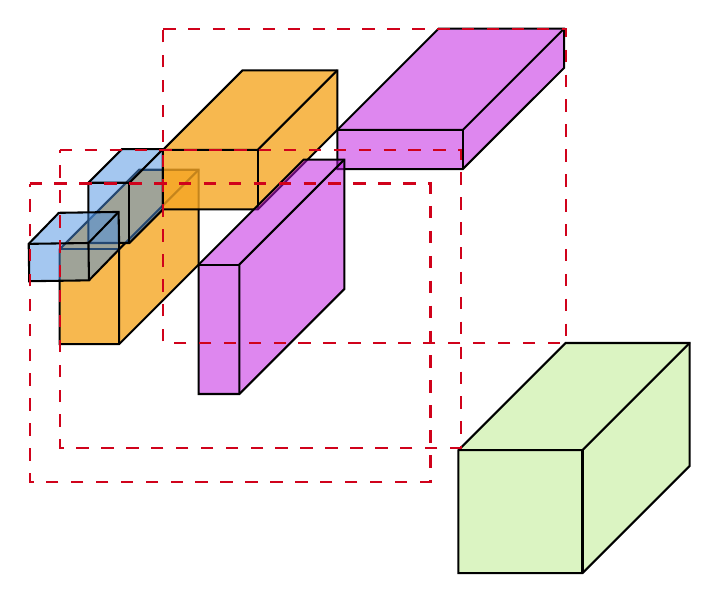
\begin{tikzpicture}[x=0.75pt,y=0.75pt,yscale=-0.7,xscale=0.7]
		%uncomment if require: \path (0,300); %set diagram left start at 0, and has height of 300
		
		%Shape: Cube [id:dp43027815424576055] 
		\draw  [fill={rgb, 255:red, 245; green, 166; blue, 35 }  ,fill opacity=0.8 ] (109.71,132.33) -- (164.43,77.61) -- (164.43,12.34) -- (123.46,12.34) -- (68.74,67.06) -- (68.74,132.33) -- cycle ; \draw   (164.43,12.34) -- (109.71,67.06) -- (109.71,132.33) ; \draw   (109.71,67.06) -- (68.74,67.06) ;
		%Shape: Cube [id:dp3746212402788034] 
		\draw  [fill={rgb, 255:red, 74; green, 144; blue, 226 }  ,fill opacity=0.5 ] (88.57,21.24) -- (111.67,-1.86) -- (139.86,-1.86) -- (139.86,39.63) -- (116.76,62.73) -- (88.57,62.73) -- cycle ; \draw   (139.86,-1.86) -- (116.76,21.24) -- (88.57,21.24) ; \draw   (116.76,21.24) -- (116.76,62.73) ;
		%Shape: Cube [id:dp8037534933597068] 
		\draw  [fill={rgb, 255:red, 245; green, 166; blue, 35 }  ,fill opacity=0.8 ] (139.86,-1.34) -- (194.59,-56.07) -- (259.86,-56.07) -- (259.86,-15.1) -- (205.14,39.63) -- (139.86,39.63) -- cycle ; \draw   (259.86,-56.07) -- (205.14,-1.34) -- (139.86,-1.34) ; \draw   (205.14,-1.34) -- (205.14,39.63) ;
		%Shape: Cube [id:dp6585637604331385] 
		\draw  [fill={rgb, 255:red, 74; green, 144; blue, 226 }  ,fill opacity=0.5 ] (88.94,88.43) -- (109.71,67.06) -- (109.33,41.36) -- (68.22,41.95) -- (47.46,63.32) -- (47.83,89.03) -- cycle ; \draw   (109.33,41.36) -- (88.57,62.73) -- (88.94,88.43) ; \draw   (88.57,62.73) -- (47.46,63.32) ;
		%Shape: Cube [id:dp42240763151438254] 
		\draw  [fill={rgb, 255:red, 184; green, 233; blue, 134 }  ,fill opacity=0.5 ] (343.2,205.32) -- (416.98,131.55) -- (502.4,131.55) -- (502.4,216.22) -- (428.62,290) -- (343.2,290) -- cycle ; \draw   (502.4,131.55) -- (428.62,205.32) -- (343.2,205.32) ; \draw   (428.62,205.32) -- (428.62,290) ;
		%Shape: Cube [id:dp9618455407010789] 
		\draw  [fill={rgb, 255:red, 189; green, 16; blue, 224 }  ,fill opacity=0.5 ] (259.86,-15.1) -- (329.52,-84.76) -- (415.93,-84.76) -- (415.93,-57.78) -- (346.27,11.87) -- (259.86,11.87) -- cycle ; \draw   (415.93,-84.76) -- (346.27,-15.1) -- (259.86,-15.1) ; \draw   (346.27,-15.1) -- (346.27,11.87) ;
		%Shape: Cube [id:dp4251536088122141] 
		\draw  [fill={rgb, 255:red, 189; green, 16; blue, 224 }  ,fill opacity=0.5 ] (192.42,166.65) -- (264.7,94.37) -- (264.7,5.33) -- (236.71,5.33) -- (164.43,77.61) -- (164.43,166.65) -- cycle ; \draw   (264.7,5.33) -- (192.42,77.61) -- (192.42,166.65) ; \draw   (192.42,77.61) -- (164.43,77.61) ;
		%Shape: Rectangle [id:dp8959103225341927] 
		\draw  [color={rgb, 255:red, 208; green, 2; blue, 27 }  ,draw opacity=1 ][dash pattern={on 4.5pt off 4.5pt}] (48.05,21.78) -- (324,21.78) -- (324,226.92) -- (48.05,226.92) -- cycle ;
		%Shape: Rectangle [id:dp5758098489109205] 
		\draw  [color={rgb, 255:red, 208; green, 2; blue, 27 }  ,draw opacity=1 ][dash pattern={on 4.5pt off 4.5pt}] (68.85,-1.42) -- (344.8,-1.42) -- (344.8,203.72) -- (68.85,203.72) -- cycle ;
		%Shape: Rectangle [id:dp8812316170269188] 
		\draw  [color={rgb, 255:red, 208; green, 2; blue, 27 }  ,draw opacity=1 ][dash pattern={on 4.5pt off 4.5pt}] (139.98,-84.76) -- (416.98,-84.76) -- (416.98,131.55) -- (139.98,131.55) -- cycle ;
		
		
		
		
	\end{tikzpicture}
	
	
	
	
	\caption{\label{fig:TI-AMSI}A pictorial demonstration of the newly added gadget for reducing from $U\otimes V\otimes W$ to $\Lambda^2(U)\otimes W$. The orange blocks correspond to the FGS gadgets in Figure~\ref{fig:3-tensor_isometry} with $\idmat_{2n+1}$. The purple blocks correspond to the FGS gadgets in Figure~\ref{fig:3-tensor_isometry} with $\idmat_{4n+2}$. The green block is the newly added alternating FGS gadget with $\idmat_{2n+1}$. Note that the green block is actually quite wide, as the frontal slices are square matrices of size $(2n+1)\cdot (N+1)$ where $N=O(\ell n+n^2)$. That is, in this picture its size is not shown proportionally.}
\end{figure}

Let $U'=\rng^{\ell+n+(2n+1)+(4n+2)+(N+1)\cdot (2n+1)}$. Let $V'=\rng^{m+N}$. We claim that $\tA$ and $\tB$ in $U\otimes V\otimes W$ are isomorphic if and only if $\bar\tA$ and $\bar\tB$ are isomorphic in $\Lambda^2(U')\otimes V'$. 

For the only if direction, we start from $(P, Q, T)\in\GL(U)\times\GL(V)\times\GL(W)$ sending $\tA$ to $\tB$ and construct $(P', T')\in \GL(U')\times \GL(V')$ sending $\bar\tA$ to $\bar\tB$. We first extend $(P, Q, T)$ to an isomorphism $(\tilde P, \tilde T)$ from $\tilde\tA$ to $\tilde\tB$ as in \cite{TI1}. In particular, $\tilde P=\diag(P, Q, U)$ and $\tilde T=\diag(T, V)$ for $V\in\GL(N, \rng)$. We then see that $\tilde T$ acts on the newly added $\tG$ gadget on the third direction. This can be remedied by introducing the congruence action of $T'$ on the first two direction as in Fact~\ref{fact:alt-FGS-tensor}.

%Note that $P$ acts on the first $m$ slices of $\tG$, so it remains to transform $\tG^P$ to $\tG$ by $P''\in \GL(m(2n+1), \rng)$ such that $\tG^P=P''^t\tG P''$. It can be verified that $P''=\begin{bmatrix}
%	\idmat_{2n+1} & 0 \\
%	0 & P^{-1}\otimes \idmat_{2n+1}
%\end{bmatrix}$ suits this purpose.

For the if direction, suppose $(P, T)\in\GL(U')\times\GL(V')$ sends $\bar \tA$ to $\bar\tB$. We first deal with the $V'$ direction. Note that the ranks of the first $m$ frontal slices of $\bar\tA$ are within $(\ell+n)\leq 2n$ as we assumed $n=\max\{n, m, \ell\}$. The ranks of the last $N$ slices are no less than $2n+1$ because of the green block in Figure~\ref{fig:TI-AMSI}.
%So the within $[2n+1, 2n+1+n+\ell]$. The ranks of the other slices are $2$. 
This ensures that in any isomorphism $(P, T)$ from $\bar\tA$ to $\bar\tB$, $T$ is of the form $\begin{bmatrix}
	T_{11} & T_{12} \\
	0 & T_{22}
\end{bmatrix}$ where $T_{11}$ is of size $m\times m$. 

We then deal with the $U'$ direction, which requires a more careful examination of the alternating FGS gadget. We first write $P\in \GL(U')$ as 
\begin{equation}\label{eq:P55}
\begin{bmatrix}
	P_{11} & P_{12} & P_{13} & P_{14} & P_{15}\\
	P_{21} & P_{22} & P_{23} & P_{24} & P_{25}\\
	P_{31} & P_{32} & P_{33} & P_{34} & P_{35}\\
	P_{41} & P_{42} & P_{43} & P_{44} & P_{45}\\
	P_{51} & P_{52} & P_{53} & P_{54} & P_{55}\\
\end{bmatrix},
\end{equation}
where $P_{11}\in\M(\ell, \rng)$, $P_{22}\in\M(n, \rng)$, $P_{33}\in\M(3n+3, \rng)$, $P_{44}\in\M(2n+1, \rng)$, and $P_{55}\in\M(N\cdot (2n+1), \rng)$. We now consider the ranks of the horizontal slices of $\bar\tA$. 
\begin{enumerate}
	\item For the first $\ell$ slices, the ranks are between $2n+1$ and $3n+1$.
	\item For the next $n$ slices, the ranks are between $4n+2$ and $5n+2$. 
	\item For the next $3n+3$ slices, they are the vertical slices of the FGS gadget, so their ranks are either $\ell$ or $n$. Recall that we set $n=\max\{\ell, m, n\}$.
	\item For the next $2n+1$ slices, they are the vertical slices of the FGS gadget, so their ranks are $N$. 
	\item For the next $N\cdot (2n+1)$ slices, they are the horizontal slices of the FGS gadget, so their ranks are $1$. 
\end{enumerate}
We first note that the ranks of (4)-slices are $N=\ell(n+1)+m(2n+2)$, which is too large, so no other slices can afford to have these added to them. It follows that $P_{4i}=0$ for $i\neq $. We then note that the ranks of (5)-slices are $1$, which is too small, so they cannot have other slices added to them. It follows that $P_{i5}=0$ for $i\neq 5$. That is, $P$ is of the form 
$$\begin{bmatrix}
	P_{11} & P_{12} & P_{13} & P_{14} & 0\\
	P_{21} & P_{22} & P_{23} & P_{24} & 0\\
	P_{31} & P_{32} & P_{33} & P_{34} & 0\\
	0 & 0 & 0 & P_{44} & 0\\
	P_{51} & P_{52} & P_{53} & P_{54} & P_{55}\\
\end{bmatrix},$$
from which we infer that $P_{44}$ and $P_{55}$ are invertible. Furthermore, 
$P'=\begin{bmatrix}
	P_{11} & P_{12} & P_{13}\\
	P_{21} & P_{22} & P_{23}\\
	P_{31} & P_{32} & P_{33}
\end{bmatrix}
$ is invertible. We can then follow the rank argument as 
in \cite[Proposition 5.1]{TI1} 
to show that 
%$P'=\begin{bmatrix}
%	P_{11} & P_{12} & 0\\
%	0 & P_{22} & 0\\
%	P_{31} & P_{32} & P_{33}
%\end{bmatrix},
$P'=\begin{bmatrix}
	P_{11} & 0 & 0\\
	0 & P_{22} & 0\\
	P_{31} & P_{32} & P_{33}
\end{bmatrix},
$ which gives that $P_{11}$ and $P_{22}$ are invertible. Now observe that the first $m$ frontal slices of $\bar\tA$ only have non-zero entries in the blue region (the original tensors), and along the $V'$ direction, $T=\begin{bmatrix}
	T_{11} & T_{12} \\
	0 & T_{22}
\end{bmatrix}$ does not bring the last $N$ slices to the first $m$ slices. These together give that $P_{11}, P_{22}, T_{11}$, which are all invertible, form an isomorphism from $\tA$ to $\tB$.
%We need to look after the newly added $\tG$ part for the $U'$ direction, which is altered by $T\in\GL(m, \rng)$, but this can be remedied by Fact~\ref{fact:alt-FGS-tensor}.
%the same argument as in \cite{TI1} follows, as we assumed $n=\max\{\ell, m, n\}$.
\end{proof}
%
%$\bar\tA\in \T(\big(\ell+n+(2n+1)+(4n+2)+(m+1)\cdot (2n+1)\big)\times\big(\ell+n+(2n+1)+(4n+2)+(m+1)\cdot (2n+1)\big)\times\big(m+(2n+1)^2+(4n+2)^2\big), \rng)$.
%
%(Note that the $\idmat_n$ in $\tilde A_{\ell+1}$ might not contribute $n$ to the rank of $\tilde A_i + \tilde A_{\ell+1}$, since it occurs in the same rows as $A_i$.) This condition is easily satisfied, for example by setting $r=\lfloor (n+m)/2 \rfloor + 1$. 

\subsubsection{From $\Lambda^2(U)\otimes V$ (resp. $\S^2(U)\otimes V$) to $\Lambda^3(U)$ (resp. $\S^3(U)$) }\label{subsec:S3U}

In this section we present reductions from $\Lambda^2(U)\otimes V$ (resp. $\S^2(U)\otimes V$) to $\Lambda^3(U)$ (resp. $\S^3(U)$). We focus on the one from $\Lambda^2(U)\otimes V$ to $\Lambda^3(U)$, as the one from $\S^2(U)\otimes V$ to $\S^3(U)$ follows the same strategy.

We first state the result formally as follows.
\begin{theorem} \label{thm:Lambda3U}
	Let $U=\rng^\ell$ and $V=\rng^m$. There is a polynomial-time algorithm $\algprobm{P}$ that takes $\tA\in \Lambda^2(U)\otimes V$ and outputs $\algprobm{P}(\tA)\in \Lambda^3(U')$ with $U'= \rng^{\ell'}$, with $\ell'=O\big((\ell+m)^3\big)$,
	%\ynote{Reminder to change this exponent later.}
	such that $\tA$ and $\tB\in \Lambda^2(U)\otimes V$ are isomorphic if and only if $\algprobm{P}(\tA)$ and $\algprobm{P}(\tB)\in \Lambda^3(U')$ are isomorphic.
	%	
	%	Tensor Isomorphism reduces to Alternating Matrix Module Isometry\ynote{Better to use alternating bilinear map isometry?} with linear blow-up. In particular, for $n \times m \times \ell$ tensors, the output is an $(\ell+1)$-dimensional space of matrices of size at most $3n+2m+2$.
\end{theorem}
\begin{proof}[Proof sketch of Theorem~\ref{thm:Lambda3U}] Over fields, a reduction from $\Lambda^2(U)\otimes V$ to $\Lambda^3(U)$ was presented in \cite{GQT}. The reduction over commutative rings makes use of some steps there but requires a further copy of the alternating FGS gadget. Here, we present a proof sketch of Theorem~\ref{thm:Lambda3U}, with an emphasis on the newly added FGS gadget. A detailed proof can be obtained without much effort by going over the proof of \cite[Proposition 4.1]{GQT}.

Let $\tA\in \Lambda^2(U)\otimes V$. We represent $\tA$ as a $3$-tensor as in Figure~\ref{fig:tA}.
\begin{figure}[!htbp]
	
	\centering
	
	
	\tikzset{every picture/.style={line width=0.75pt}} %set default line width to 0.75pt        
	
	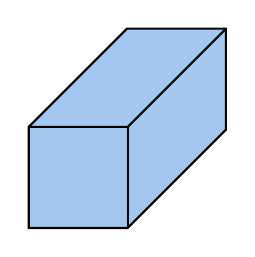
\begin{tikzpicture}[x=0.75pt,y=0.75pt,yscale=-1,xscale=1]
		%uncomment if require: \path (0,300); %set diagram left start at 0, and has height of 300
		
		%Shape: Cube [id:dp9961265448984828] 
		\draw  [fill={rgb, 255:red, 74; green, 144; blue, 226 }  ,fill opacity=0.5 ] (69.33,120.76) -- (116.63,73.47) -- (164.33,73.47) -- (164.33,122.17) -- (117.04,169.47) -- (69.33,169.47) -- cycle ; \draw   (164.33,73.47) -- (117.04,120.76) -- (69.33,120.76) ; \draw   (117.04,120.76) -- (117.04,169.47) ;
		
		
		
		
	\end{tikzpicture}
	
	\caption{\label{fig:tA}A pictorial demonstration of $\tA\in \Lambda^2(U)\otimes V$.}
\end{figure}

The first step is to make a tensor that is alternating in three directions. This is done by setting a $2\times 2\times 2$ block tensor, with rotated $\tA$ in the $(1, 1, 2)$ and $(1, 2, 1)$ positions, and $-\tA$ in the $(2, 1, 1)$ position. Thus we get a tensor $\tilde\tA$ in Figure~\ref{fig:3tA}.


\begin{figure}[!htbp]

\centering


\tikzset{every picture/.style={line width=0.75pt}} %set default line width to 0.75pt        

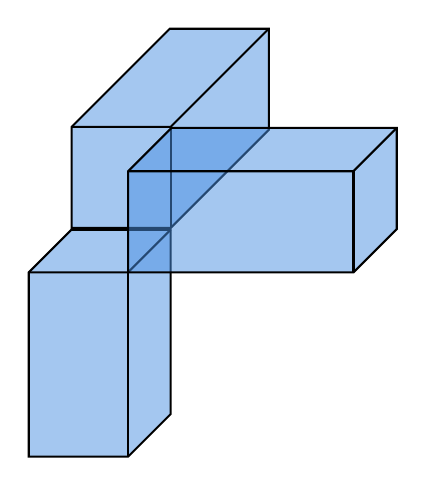
\begin{tikzpicture}[x=0.75pt,y=0.75pt,yscale=-1,xscale=1]
	%uncomment if require: \path (0,300); %set diagram left start at 0, and has height of 300
	
	%Shape: Cube [id:dp5325535269556623] 
	\draw  [fill={rgb, 255:red, 74; green, 144; blue, 226 }  ,fill opacity=0.5 ] (234.67,115.76) -- (281.96,68.47) -- (329.67,68.47) -- (329.67,117.17) -- (282.37,164.47) -- (234.67,164.47) -- cycle ; \draw   (329.67,68.47) -- (282.37,115.76) -- (234.67,115.76) ; \draw   (282.37,115.76) -- (282.37,164.47) ;
	%Shape: Cube [id:dp08184821646409679] 
	\draw  [fill={rgb, 255:red, 74; green, 144; blue, 226 }  ,fill opacity=0.5 ] (214,185.84) -- (234.51,165.33) -- (282.37,165.33) -- (282.37,254.16) -- (261.86,274.67) -- (214,274.67) -- cycle ; \draw   (282.37,165.33) -- (261.86,185.84) -- (214,185.84) ; \draw   (261.86,185.84) -- (261.86,274.67) ;
	%Shape: Cube [id:dp8106035381253227] 
	\draw  [fill={rgb, 255:red, 74; green, 144; blue, 226 }  ,fill opacity=0.5 ] (261.86,137.14) -- (282.73,116.27) -- (391.33,116.27) -- (391.33,164.97) -- (370.46,185.84) -- (261.86,185.84) -- cycle ; \draw   (391.33,116.27) -- (370.46,137.14) -- (261.86,137.14) ; \draw   (370.46,137.14) -- (370.46,185.84) ;
	
	
	
	
\end{tikzpicture}


\caption{\label{fig:3tA}A pictorial demonstration of an alternating tensor $\tilde\tA$ from $\tA\in \Lambda^2(U)\otimes V$.}
\end{figure}

The second step is to install the alternating FGS tensor $\tG=\tG_{\ell+m+1, \ell}$ to $\tilde\tA$, with three copies appropriately rotated and signed, as shown in Figure~\ref{fig:3tA_FGS}.


\begin{figure}[!htbp]
	
	\centering


\tikzset{every picture/.style={line width=0.75pt}} %set default line width to 0.75pt        
\resizebox{7cm}{!}{
	
	
	\tikzset{every picture/.style={line width=0.75pt}} %set default line width to 0.75pt        
	
	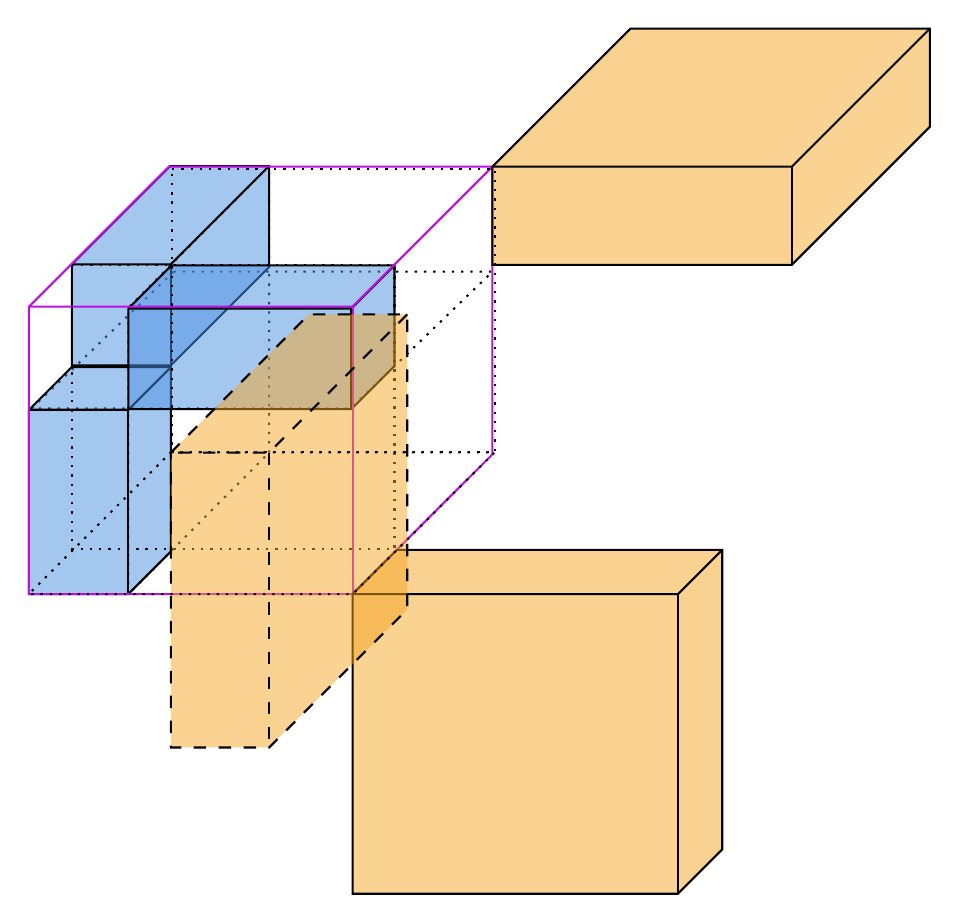
\begin{tikzpicture}[x=0.75pt,y=0.75pt,yscale=-1,xscale=1]
		%uncomment if require: \path (0,300); %set diagram left start at 0, and has height of 300
		
		%Shape: Parallelogram [id:dp5359170435102052] 
		\draw  [dash pattern={on 0.84pt off 2.51pt}] (158.24,-9.72) -- (311.84,-9.72) -- (243.56,56.11) -- (89.96,56.11) -- cycle ;
		%Shape: Parallelogram [id:dp6877235911913138] 
		\draw  [dash pattern={on 0.84pt off 2.51pt}] (204.2,77.48) -- (204.2,-60.56) -- (136.39,7.6) -- (136.39,145.64) -- cycle ;
		%Shape: Cube [id:dp13594938626002495] 
		\draw  [fill={rgb, 255:red, 74; green, 144; blue, 226 }  ,fill opacity=0.5 ] (109.2,-13.26) -- (156.5,-60.56) -- (204.2,-60.56) -- (204.2,-11.85) -- (156.9,35.44) -- (109.2,35.44) -- cycle ; \draw   (204.2,-60.56) -- (156.9,-13.26) -- (109.2,-13.26) ; \draw   (156.9,-13.26) -- (156.9,35.44) ;
		%Shape: Cube [id:dp4594421272022775] 
		\draw  [fill={rgb, 255:red, 74; green, 144; blue, 226 }  ,fill opacity=0.5 ] (88.53,56.82) -- (109.04,36.31) -- (156.9,36.31) -- (156.9,125.13) -- (136.39,145.64) -- (88.53,145.64) -- cycle ; \draw   (156.9,36.31) -- (136.39,56.82) -- (88.53,56.82) ; \draw   (136.39,56.82) -- (136.39,145.64) ;
		%Shape: Cube [id:dp9838274328728649] 
		\draw  [fill={rgb, 255:red, 74; green, 144; blue, 226 }  ,fill opacity=0.5 ] (136.39,8.03) -- (157.18,-12.76) -- (264.64,-12.76) -- (264.64,35.74) -- (243.86,56.52) -- (136.39,56.52) -- cycle ; \draw   (264.64,-12.76) -- (243.86,8.03) -- (136.39,8.03) ; \draw   (243.86,8.03) -- (243.86,56.52) ;
		%Shape: Cube [id:dp9525735963151862] 
		\draw  [color={rgb, 255:red, 189; green, 16; blue, 224 }  ,draw opacity=1 ] (88.53,7.11) -- (155.92,-60.28) -- (311.84,-60.28) -- (311.84,78.26) -- (244.45,145.64) -- (88.53,145.64) -- cycle ; \draw  [color={rgb, 255:red, 189; green, 16; blue, 224 }  ,draw opacity=1 ] (311.84,-60.28) -- (244.45,7.11) -- (88.53,7.11) ; \draw  [color={rgb, 255:red, 189; green, 16; blue, 224 }  ,draw opacity=1 ] (244.45,7.11) -- (244.45,145.64) ;
		%Shape: Rectangle [id:dp6171797020228431] 
		\draw  [dash pattern={on 0.84pt off 2.51pt}] (109.2,-12.76) -- (264.64,-12.76) -- (264.64,123.88) -- (109.2,123.88) -- cycle ;
		%Shape: Cube [id:dp572143672202565] 
		\draw  [fill={rgb, 255:red, 245; green, 166; blue, 35 }  ,fill opacity=0.5 ] (244.45,145.64) -- (265.81,124.29) -- (422.56,124.29) -- (422.56,268.64) -- (401.2,290) -- (244.45,290) -- cycle ; \draw   (422.56,124.29) -- (401.2,145.64) -- (244.45,145.64) ; \draw   (401.2,145.64) -- (401.2,290) ;
		%Shape: Cube [id:dp8222824172232956] 
		\draw  [fill={rgb, 255:red, 245; green, 166; blue, 35 }  ,fill opacity=0.5 ] (311.84,-60.28) -- (378.33,-126.77) -- (522.56,-126.77) -- (522.56,-79.5) -- (456.07,-13.01) -- (311.84,-13.01) -- cycle ; \draw   (522.56,-126.77) -- (456.07,-60.28) -- (311.84,-60.28) ; \draw   (456.07,-60.28) -- (456.07,-13.01) ;
		%Shape: Cube [id:dp27636218363218745] 
		\draw  [fill={rgb, 255:red, 245; green, 166; blue, 35 }  ,fill opacity=0.5 ][dash pattern={on 4.5pt off 4.5pt}] (156.87,77.48) -- (223.45,10.9) -- (270.79,10.9) -- (270.79,152.95) -- (204.2,219.54) -- (156.87,219.54) -- cycle ; \draw  [dash pattern={on 4.5pt off 4.5pt}] (270.79,10.9) -- (204.2,77.48) -- (156.87,77.48) ; \draw  [dash pattern={on 4.5pt off 4.5pt}] (204.2,77.48) -- (204.2,219.54) ;
		%Shape: Rectangle [id:dp7766772894732206] 
		\draw  [dash pattern={on 0.84pt off 2.51pt}] (156.88,77.32) -- (312.91,77.32) -- (244.45,145.64) -- (88.41,145.64) -- cycle ;
		%Shape: Rectangle [id:dp8404831100530714] 
		\draw  [dash pattern={on 0.84pt off 2.51pt}] (157.47,-59.32) -- (312.91,-59.32) -- (312.91,77.32) -- (157.47,77.32) -- cycle ;
		
		
		
		
	\end{tikzpicture}
	
}

\caption{\label{fig:3tA_FGS}A pictorial demonstration of installing three alternating FGS tensors to  $\tilde\tA$ as in \cite{GQT}. Here, the FGS tensors are in orange colors, and unfilled entries are all $0$. They are appopriately rotated to match the sizes. The front tensor is also multiplied with $-1$.}
\end{figure}

The construction as in Figure~\ref{fig:3tA_FGS} works over the field setting. It makes the assumption that the frontal slices of $\tA$ are linearly independent. To remove this assumption, we need to first add three copies of $\tG_{2(\ell+m+1), m}$, appropriately rotated and signed, as in Figure~\ref{fig:3tA_2FGS}. 


\begin{figure}[!htbp]
	
	\centering
	
	
	
	\tikzset{every picture/.style={line width=0.75pt}} %set default line width to 0.75pt        
	\resizebox{10cm}{!}{
		
%		\tikzset{every picture/.style={line width=0.75pt}} %set default line width to 0.75pt        
		
	
	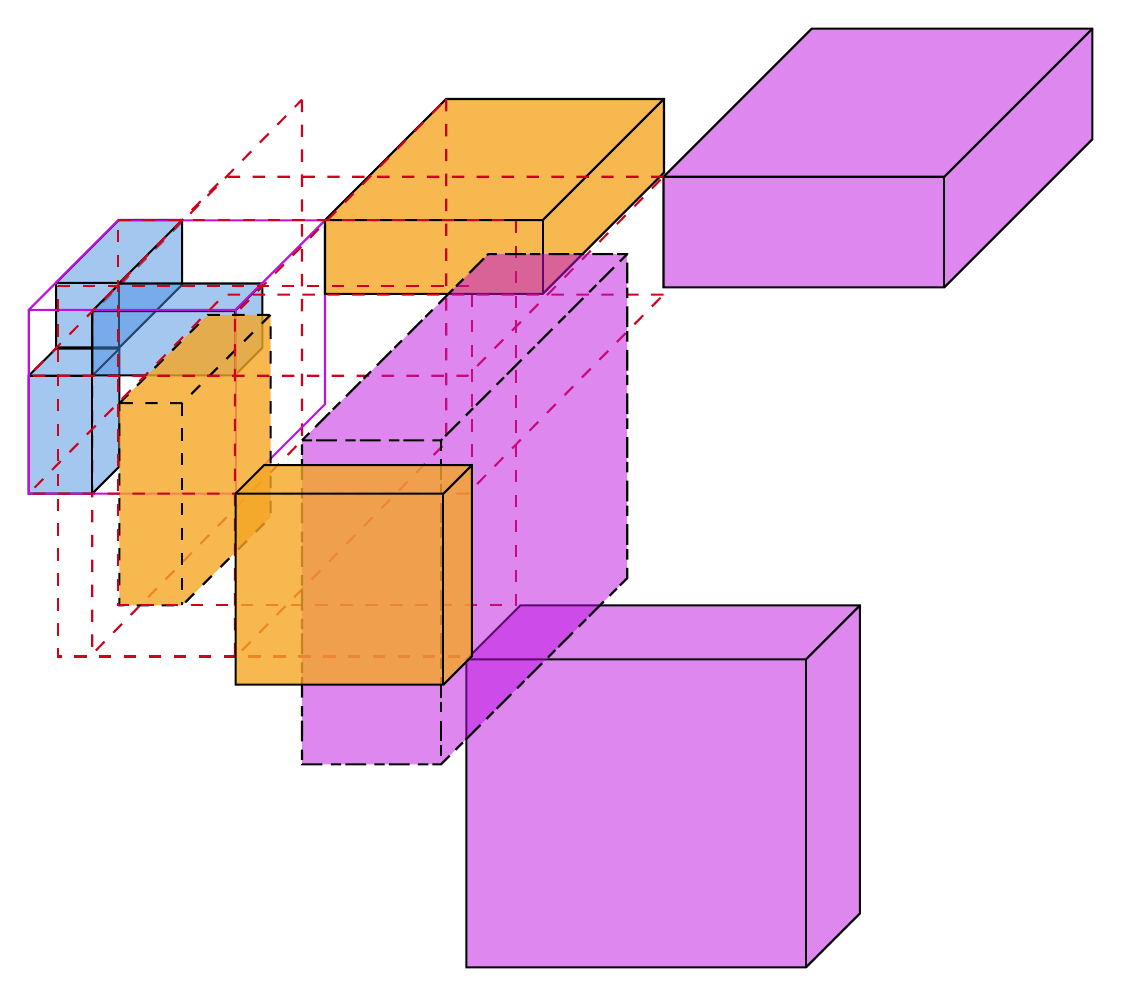
\begin{tikzpicture}[x=0.75pt,y=0.75pt,yscale=-1,xscale=1]
		%uncomment if require: \path (0,300); %set diagram left start at 0, and has height of 300
		
		%Shape: Rectangle [id:dp5529640108812919] 
		\draw  [color={rgb, 255:red, 208; green, 2; blue, 27 }  ,draw opacity=1 ][dash pattern={on 4.5pt off 4.5pt}] (240.16,-128.08) -- (240.16,36.06) -- (139.09,139.1) -- (139.09,-25.05) -- cycle ;
		%Shape: Cube [id:dp4918426294628846] 
		\draw  [fill={rgb, 255:red, 74; green, 144; blue, 226 }  ,fill opacity=0.5 ] (121.7,-39.83) -- (151.94,-70.07) -- (182.44,-70.07) -- (182.44,-38.93) -- (152.2,-8.69) -- (121.7,-8.69) -- cycle ; \draw   (182.44,-70.07) -- (152.2,-39.83) -- (121.7,-39.83) ; \draw   (152.2,-39.83) -- (152.2,-8.69) ;
		%Shape: Cube [id:dp44782835373726115] 
		\draw  [fill={rgb, 255:red, 74; green, 144; blue, 226 }  ,fill opacity=0.5 ] (108.49,4.97) -- (121.6,-8.14) -- (152.2,-8.14) -- (152.2,48.65) -- (139.09,61.76) -- (108.49,61.76) -- cycle ; \draw   (152.2,-8.14) -- (139.09,4.97) -- (108.49,4.97) ; \draw   (139.09,4.97) -- (139.09,61.76) ;
		%Shape: Cube [id:dp1355731701358771] 
		\draw  [fill={rgb, 255:red, 74; green, 144; blue, 226 }  ,fill opacity=0.5 ] (139.09,-26.22) -- (152.37,-39.51) -- (221.08,-39.51) -- (221.08,-8.51) -- (207.79,4.78) -- (139.09,4.78) -- cycle ; \draw   (221.08,-39.51) -- (207.79,-26.22) -- (139.09,-26.22) ; \draw   (207.79,-26.22) -- (207.79,4.78) ;
		%Shape: Cube [id:dp33750438991152487] 
		\draw  [color={rgb, 255:red, 189; green, 16; blue, 224 }  ,draw opacity=1 ] (108.49,-26.81) -- (151.57,-69.89) -- (251.25,-69.89) -- (251.25,18.68) -- (208.17,61.76) -- (108.49,61.76) -- cycle ; \draw  [color={rgb, 255:red, 189; green, 16; blue, 224 }  ,draw opacity=1 ] (251.25,-69.89) -- (208.17,-26.81) -- (108.49,-26.81) ; \draw  [color={rgb, 255:red, 189; green, 16; blue, 224 }  ,draw opacity=1 ] (208.17,-26.81) -- (208.17,61.76) ;
		%Shape: Cube [id:dp7826463862036612] 
		\draw  [fill={rgb, 255:red, 245; green, 166; blue, 35 }  ,fill opacity=0.8 ] (251.25,-70) -- (309.65,-128.4) -- (414.56,-128.4) -- (414.56,-92.93) -- (356.16,-34.53) -- (251.25,-34.53) -- cycle ; \draw   (414.56,-128.4) -- (356.16,-70) -- (251.25,-70) ; \draw   (356.16,-70) -- (356.16,-34.53) ;
		%Shape: Cube [id:dp6855989926227026] 
		\draw  [fill={rgb, 255:red, 245; green, 166; blue, 35 }  ,fill opacity=0.8 ][dash pattern={on 4.5pt off 4.5pt}] (152.18,18.18) -- (194.75,-24.39) -- (225.01,-24.39) -- (225.01,73.03) -- (182.44,115.6) -- (152.18,115.6) -- cycle ; \draw  [dash pattern={on 4.5pt off 4.5pt}] (225.01,-24.39) -- (182.44,18.18) -- (152.18,18.18) ; \draw  [dash pattern={on 4.5pt off 4.5pt}] (182.44,18.18) -- (182.44,115.6) ;
		%Shape: Rectangle [id:dp6526214782114248] 
		\draw  [color={rgb, 255:red, 208; green, 2; blue, 27 }  ,draw opacity=1 ][dash pattern={on 4.5pt off 4.5pt}] (122.45,-38.5) -- (322.04,-38.5) -- (322.04,140.21) -- (122.45,140.21) -- cycle ;
		%Shape: Rectangle [id:dp19557597977127683] 
		\draw  [color={rgb, 255:red, 208; green, 2; blue, 27 }  ,draw opacity=1 ][dash pattern={on 4.5pt off 4.5pt}] (151.57,-69.89) -- (343.36,-69.89) -- (343.36,115.6) -- (151.57,115.6) -- cycle ;
		%Shape: Cube [id:dp039294912967351436] 
		\draw  [fill={rgb, 255:red, 189; green, 16; blue, 224 }  ,fill opacity=0.5 ] (319.36,141.58) -- (345.34,115.6) -- (508.96,115.6) -- (508.96,264.02) -- (482.98,290) -- (319.36,290) -- cycle ; \draw   (508.96,115.6) -- (482.98,141.58) -- (319.36,141.58) ; \draw   (482.98,141.58) -- (482.98,290) ;
		%Shape: Cube [id:dp14616073549525388] 
		\draw  [fill={rgb, 255:red, 189; green, 16; blue, 224 }  ,fill opacity=0.5 ] (414.34,-90.91) -- (485.67,-162.25) -- (620.96,-162.25) -- (620.96,-108.99) -- (549.63,-37.65) -- (414.34,-37.65) -- cycle ; \draw   (620.96,-162.25) -- (549.63,-90.91) -- (414.34,-90.91) ; \draw   (549.63,-90.91) -- (549.63,-37.65) ;
		%Shape: Rectangle [id:dp646903937214302] 
		\draw  [color={rgb, 255:red, 208; green, 2; blue, 27 }  ,draw opacity=1 ][dash pattern={on 4.5pt off 4.5pt}] (309.65,-128.4) -- (309.65,36.99) -- (207.79,140.83) -- (207.79,-24.56) -- cycle ;
		%Shape: Rectangle [id:dp45546662267679894] 
		\draw  [color={rgb, 255:red, 208; green, 2; blue, 27 }  ,draw opacity=1 ][dash pattern={on 4.5pt off 4.5pt}] (414.34,-90.91) -- (202.89,-90.91) -- (108.49,4.97) -- (319.94,4.97) -- cycle ;
		%Shape: Rectangle [id:dp023548941603051654] 
		\draw  [color={rgb, 255:red, 208; green, 2; blue, 27 }  ,draw opacity=1 ][dash pattern={on 4.5pt off 4.5pt}] (414.34,-34.12) -- (202.89,-34.12) -- (108.49,61.76) -- (319.94,61.76) -- cycle ;
		%Shape: Cube [id:dp5455096928499541] 
		\draw  [fill={rgb, 255:red, 189; green, 16; blue, 224 }  ,fill opacity=0.5 ][dash pattern={on 3.75pt off 3pt on 7.5pt off 1.5pt}] (240.16,36.06) -- (329.88,-53.65) -- (396.86,-53.65) -- (396.86,102.49) -- (307.14,192.21) -- (240.16,192.21) -- cycle ; \draw  [dash pattern={on 3.75pt off 3pt on 7.5pt off 1.5pt}] (396.86,-53.65) -- (307.14,36.06) -- (240.16,36.06) ; \draw  [dash pattern={on 3.75pt off 3pt on 7.5pt off 1.5pt}] (307.14,36.06) -- (307.14,192.21) ;
		%Shape: Cube [id:dp8343104534811807] 
		\draw  [fill={rgb, 255:red, 245; green, 166; blue, 35 }  ,fill opacity=0.8 ] (208.17,61.76) -- (221.91,48.02) -- (322.04,48.02) -- (322.04,140.02) -- (308.31,153.76) -- (208.17,153.76) -- cycle ; \draw   (322.04,48.02) -- (308.31,61.76) -- (208.17,61.76) ; \draw   (308.31,61.76) -- (308.31,153.76) ;
		
		
		
		
	\end{tikzpicture}
		
}




\caption{\label{fig:3tA_2FGS}A pictorial demonstration of installing three more alternating FGS tensors to  $\tilde\tA$. Here, the newly added FGS tensors are in purple colors, and unfilled entries are all $0$. They are appopriately rotated to match the sizes. The front tensor is also multiplied with $-1$.}
\end{figure}

After this step, let $N=
(\ell+1)\cdot(\ell+m+1)+(m+1)\cdot(2\ell+2m+2)$ be the sum of the sizes of the frontal slices of the two added alternating FGS gadgets. We then add further alternating FGS gadgets $\tG_{4(\ell+m+1), N}$ to the three directions as shown in Figure~\ref{fig:3tA_3FGS}.

\begin{figure}[!htbp]
	
	\centering
	
	
	
	
	\tikzset{every picture/.style={line width=0.75pt}} %set default line width to 0.75pt        
	
	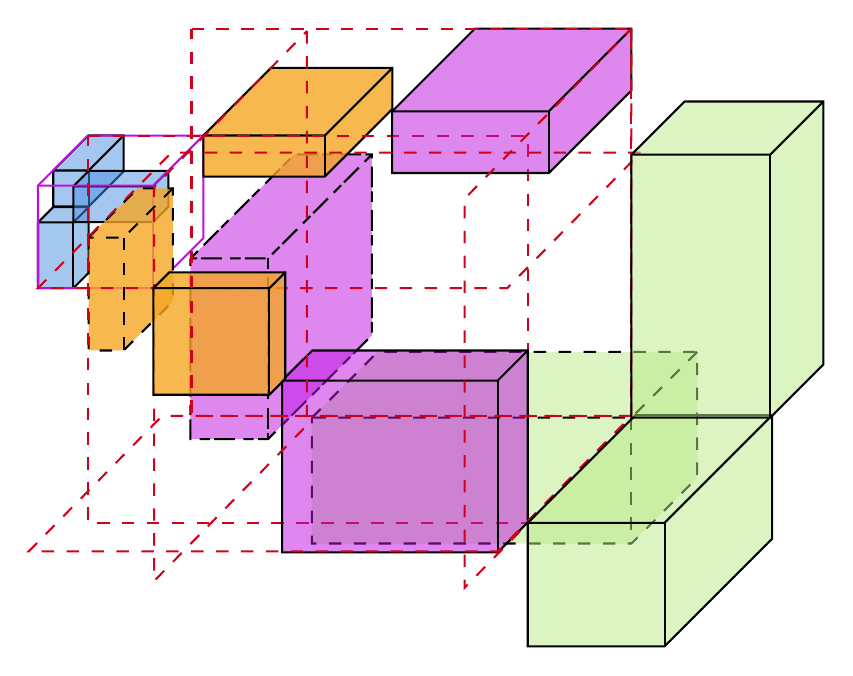
\begin{tikzpicture}[x=0.75pt,y=0.75pt,yscale=-1,xscale=1]
		%uncomment if require: \path (0,300); %set diagram left start at 0, and has height of 300
		
		%Shape: Cube [id:dp10910261260416076] 
		\draw  [fill={rgb, 255:red, 184; green, 233; blue, 134 }  ,fill opacity=0.5 ][dash pattern={on 4.5pt off 4.5pt}] (197.28,179.79) -- (228.97,148.1) -- (382.9,148.1) -- (382.9,208.76) -- (351.22,240.45) -- (197.28,240.45) -- cycle ; \draw  [dash pattern={on 4.5pt off 4.5pt}] (382.9,148.1) -- (351.22,179.79) -- (197.28,179.79) ; \draw  [dash pattern={on 4.5pt off 4.5pt}] (351.22,179.79) -- (351.22,240.45) ;
		%Shape: Cube [id:dp010407458430554017] 
		\draw  [fill={rgb, 255:red, 189; green, 16; blue, 224 }  ,fill opacity=0.5 ][dash pattern={on 3.75pt off 3pt on 7.5pt off 1.5pt}] (138.75,103.05) -- (188.81,52.99) -- (226.18,52.99) -- (226.18,140.11) -- (176.13,190.17) -- (138.75,190.17) -- cycle ; \draw  [dash pattern={on 3.75pt off 3pt on 7.5pt off 1.5pt}] (226.18,52.99) -- (176.13,103.05) -- (138.75,103.05) ; \draw  [dash pattern={on 3.75pt off 3pt on 7.5pt off 1.5pt}] (176.13,103.05) -- (176.13,190.17) ;
		%Shape: Cube [id:dp2212926307158285] 
		\draw  [fill={rgb, 255:red, 74; green, 144; blue, 226 }  ,fill opacity=0.5 ] (72.66,60.71) -- (89.53,43.83) -- (106.55,43.83) -- (106.55,61.21) -- (89.68,78.08) -- (72.66,78.08) -- cycle ; \draw   (106.55,43.83) -- (89.68,60.71) -- (72.66,60.71) ; \draw   (89.68,60.71) -- (89.68,78.08) ;
		%Shape: Cube [id:dp3336413425371043] 
		\draw  [fill={rgb, 255:red, 74; green, 144; blue, 226 }  ,fill opacity=0.5 ] (65.29,85.7) -- (72.61,78.39) -- (89.68,78.39) -- (89.68,110.07) -- (82.36,117.39) -- (65.29,117.39) -- cycle ; \draw   (89.68,78.39) -- (82.36,85.7) -- (65.29,85.7) ; \draw   (82.36,85.7) -- (82.36,117.39) ;
		%Shape: Cube [id:dp35521366779056507] 
		\draw  [fill={rgb, 255:red, 74; green, 144; blue, 226 }  ,fill opacity=0.5 ] (82.36,68.3) -- (89.78,60.89) -- (128.11,60.89) -- (128.11,78.18) -- (120.69,85.6) -- (82.36,85.6) -- cycle ; \draw   (128.11,60.89) -- (120.69,68.3) -- (82.36,68.3) ; \draw   (120.69,68.3) -- (120.69,85.6) ;
		%Shape: Cube [id:dp30428746453802] 
		\draw  [color={rgb, 255:red, 189; green, 16; blue, 224 }  ,draw opacity=1 ] (65.29,67.97) -- (89.33,43.93) -- (144.94,43.93) -- (144.94,93.35) -- (120.91,117.39) -- (65.29,117.39) -- cycle ; \draw  [color={rgb, 255:red, 189; green, 16; blue, 224 }  ,draw opacity=1 ] (144.94,43.93) -- (120.91,67.97) -- (65.29,67.97) ; \draw  [color={rgb, 255:red, 189; green, 16; blue, 224 }  ,draw opacity=1 ] (120.91,67.97) -- (120.91,117.39) ;
		%Shape: Cube [id:dp2747072360248086] 
		\draw  [fill={rgb, 255:red, 245; green, 166; blue, 35 }  ,fill opacity=0.8 ] (144.94,43.87) -- (177.53,11.29) -- (236.06,11.29) -- (236.06,31.08) -- (203.47,63.66) -- (144.94,63.66) -- cycle ; \draw   (236.06,11.29) -- (203.47,43.87) -- (144.94,43.87) ; \draw   (203.47,43.87) -- (203.47,63.66) ;
		%Shape: Cube [id:dp10777045047168898] 
		\draw  [fill={rgb, 255:red, 245; green, 166; blue, 35 }  ,fill opacity=0.8 ][dash pattern={on 4.5pt off 4.5pt}] (89.66,93.07) -- (113.42,69.32) -- (130.3,69.32) -- (130.3,123.68) -- (106.55,147.43) -- (89.66,147.43) -- cycle ; \draw  [dash pattern={on 4.5pt off 4.5pt}] (130.3,69.32) -- (106.55,93.07) -- (89.66,93.07) ; \draw  [dash pattern={on 4.5pt off 4.5pt}] (106.55,93.07) -- (106.55,147.43) ;
		%Shape: Rectangle [id:dp23057727830539432] 
		\draw  [color={rgb, 255:red, 208; green, 2; blue, 27 }  ,draw opacity=1 ][dash pattern={on 4.5pt off 4.5pt}] (89.33,43.93) -- (301.28,43.93) -- (301.28,230.49) -- (89.33,230.49) -- cycle ;
		%Shape: Cube [id:dp4673558879684805] 
		\draw  [fill={rgb, 255:red, 189; green, 16; blue, 224 }  ,fill opacity=0.5 ] (182.94,161.92) -- (197.44,147.43) -- (301.28,147.43) -- (301.28,230.23) -- (286.78,244.73) -- (182.94,244.73) -- cycle ; \draw   (301.28,147.43) -- (286.78,161.92) -- (182.94,161.92) ; \draw   (286.78,161.92) -- (286.78,244.73) ;
		%Shape: Cube [id:dp8733928889072688] 
		\draw  [fill={rgb, 255:red, 189; green, 16; blue, 224 }  ,fill opacity=0.5 ] (235.94,32.21) -- (275.74,-7.59) -- (351.22,-7.59) -- (351.22,22.12) -- (311.42,61.92) -- (235.94,61.92) -- cycle ; \draw   (351.22,-7.59) -- (311.42,32.21) -- (235.94,32.21) ; \draw   (311.42,32.21) -- (311.42,61.92) ;
		%Shape: Rectangle [id:dp9618704757003733] 
		\draw  [color={rgb, 255:red, 208; green, 2; blue, 27 }  ,draw opacity=1 ][dash pattern={on 4.5pt off 4.5pt}] (194.88,-6.4) -- (194.88,183.46) -- (121.28,258.49) -- (121.28,68.63) -- cycle ;
		%Shape: Rectangle [id:dp5797033001671397] 
		\draw  [color={rgb, 255:red, 208; green, 2; blue, 27 }  ,draw opacity=1 ][dash pattern={on 4.5pt off 4.5pt}] (355.68,52.09) -- (129.58,52.09) -- (65.3,117.39) -- (291.4,117.39) -- cycle ;
		%Shape: Cube [id:dp5624338302910918] 
		\draw  [fill={rgb, 255:red, 245; green, 166; blue, 35 }  ,fill opacity=0.8 ] (120.91,117.43) -- (128.57,109.77) -- (184.44,109.77) -- (184.44,161.1) -- (176.78,168.76) -- (120.91,168.76) -- cycle ; \draw   (184.44,109.77) -- (176.78,117.43) -- (120.91,117.43) ; \draw   (176.78,117.43) -- (176.78,168.76) ;
		%Shape: Rectangle [id:dp0236785549550933] 
		\draw  [color={rgb, 255:red, 208; green, 2; blue, 27 }  ,draw opacity=1 ][dash pattern={on 4.5pt off 4.5pt}] (139.27,-7.59) -- (351.22,-7.59) -- (351.22,178.96) -- (139.27,178.96) -- cycle ;
		%Shape: Rectangle [id:dp5318037279947354] 
		\draw  [color={rgb, 255:red, 208; green, 2; blue, 27 }  ,draw opacity=1 ][dash pattern={on 4.5pt off 4.5pt}] (351.22,178.96) -- (125.12,178.96) -- (60.83,244.26) -- (286.93,244.26) -- cycle ;
		%Shape: Rectangle [id:dp4505524623612511] 
		\draw  [color={rgb, 255:red, 208; green, 2; blue, 27 }  ,draw opacity=1 ][dash pattern={on 4.5pt off 4.5pt}] (351.22,-7.59) -- (351.22,179.79) -- (270.88,261.69) -- (270.88,74.3) -- cycle ;
		%Shape: Cube [id:dp8462432789678338] 
		\draw  [fill={rgb, 255:red, 184; green, 233; blue, 134 }  ,fill opacity=0.5 ] (301.28,230.49) -- (353.13,178.63) -- (419.03,178.63) -- (419.03,238.15) -- (367.17,290) -- (301.28,290) -- cycle ; \draw   (419.03,178.63) -- (367.17,230.49) -- (301.28,230.49) ; \draw   (367.17,230.49) -- (367.17,290) ;
		%Shape: Cube [id:dp6692306998427315] 
		\draw  [fill={rgb, 255:red, 184; green, 233; blue, 134 }  ,fill opacity=0.5 ] (351.22,53.08) -- (376.82,27.48) -- (443.68,27.48) -- (443.68,154.19) -- (418.08,179.79) -- (351.22,179.79) -- cycle ; \draw   (443.68,27.48) -- (418.08,53.08) -- (351.22,53.08) ; \draw   (418.08,53.08) -- (418.08,179.79) ;
		
		
		
		
	\end{tikzpicture}
	
	
	\caption{\label{fig:3tA_3FGS}A pictorial demonstration of installing further three more alternating FGS tensors to  $\tilde\tA$. Here, the newly added FGS tensors are in green colors, and unfilled entries are all $0$. They are appopriately rotated to match the sizes. The front tensor is also multiplied with $-1$. Note that the frontal slices of the newly added FGS tensors are of size $(N+1)\cdot 4(\ell+m+1)=O((\ell+m)^3)$, so the green blocks are actually quite wide, which is not shown proportionally in the picture.}
\end{figure}


Let $U'=\rng^{\ell+m+N+(N+1)\cdot 4(\ell+m+1)}$. Let the resulting alternating tensor from the above process be $\bar\tA$. We need to show that $\tA$ and $\tB$ are isomorphic as in $\Lambda^2(U)\otimes V$ if and only if $\bar\tA$ and $\bar\tB$ are isomorphic as in $\Lambda^3(U')$.

\paragraph{The if direction.} Recall that $U'=\rng^{\ell+m+N+(N+1)\cdot 4(\ell+m+1)}$. For the if direction, suppose $\bar\tA$ and $\bar\tB$ are isomorphic as in $\Lambda^3(U')$ via 
$$P=\begin{bmatrix}
	P_{11} & P_{12} & P_{13} & P_{14} & P_{15}\\
	P_{21} & P_{22} & P_{23} & P_{24} & P_{25}\\
	P_{31} & P_{32} & P_{33} & P_{34} & P_{35}\\
	P_{41} & P_{42} & P_{43} & P_{44} & P_{45}\\
	P_{51} & P_{52} & P_{53} & P_{54} & P_{55}\\
\end{bmatrix},$$
where $P_{11}$ is of size $\ell\times \ell$, $P_{22}$ is of size $m\times m$, $P_{33}$ is of size $N\times N$, $P_{44}$ is of size $4(\ell+m+1)\times4(\ell+m+1)$, and $P_{55}$ is of size $4N(\ell+m+1)\times 4N(\ell+m+1)$. We then examine the ranks of the frontal slices.
\begin{enumerate}
	\item For the first $\ell$ slices, their ranks are between $2(\ell+m+1)$ and $2(\ell+m+1)+\ell+m$.
	\item For the next $m$ slices, their ranks are between $4(\ell+m+1)$ and $4(\ell+m+1)+\ell+m$. 
	
%	Also note that the rank of any non-zero linear combination is between $6(\ell+m+1)+\ell+m$.
	\item For the next $N$ slices, their ranks are between $8(\ell+m+1)$ and $8(\ell+m+1)+2(\ell+m)$.
	
	\item For the next $4(\ell+m+1)$ slices, their ranks are $2N=\Theta((\ell+m)^2)$. 
	
	\item For the last few slices, their ranks are $2$.
\end{enumerate}
Because of these rank statistics, by an analysis similar to that after Equation~\ref{eq:P55}, we obtain that $P$ is of the form 
\begin{equation}\label{eq:P-form}
	\begin{bmatrix}
	P_{11} & 0 & 0 & 0 & 0\\
	0 & P_{22} & 0 & 0 & 0\\
	0 & 0 & P_{33} & 0 & 0\\
	0 & 0 & 0 & P_{44} & 0\\
	P_{51} & P_{52} & P_{53} & P_{54} & P_{55}\\
\end{bmatrix}.
\end{equation}

We claim that the $(1, 1, 2)$ block of $P^t\bar\tA^P P$ is $P_{11}^t\tA^{P_{22}}P_{11}$. If this claim holds, then by $P$ sending $\bar\tA$ to $\bar\tB$, we have $P_{11}^t\tA^{P_{22}}P_{11}=\tB$, showing that $\tA$ and $\tB$ are isomorphic in $\Lambda^2(U)\otimes V$.

We first examine how a matrix $P$ in the form of Equation~\ref{eq:P-form} acts on the frontal slices with indices in $[\ell+1, \ell+m]$. Note that the frontal slices in this range are of the form. 
$S=\begin{bmatrix}
	S_{11} & & & & \\
	& & & & \\
	& & S_{33} & & \\
	& & & & \\
	& & & & 
\end{bmatrix}$. Therefore, $\tilde S:=P^tSP=\begin{bmatrix}
P_{11}^tS_{11}P_{11} & & & & \\
& & & & \\
& & P_{33}^tS_{33}P_{33} & & \\
& & & & \\
& & & & 
\end{bmatrix}$. 

Then consider the action of $P$ on the third direction in the $(1, 1)$ direction, which consists of $(1, 1, i)$ blocks where $i\in[5]$. By the form of $P$ in Equation~\ref{eq:FGS-horizontal}, the resulting $(1, 1, 2)$ block is a linear combination of the $(1, 1, 2)$ block and the $(1, 1, 5)$ block. Consider the $(1, 1, 5)$ block of $P^t\bar\tA P$. As the last $4N(\ell+m+1)$ frontal slices are of the form $T=\begin{bmatrix}
	& & & & \\
	& & & & \\
	& & & T_{34} & T_{35}\\
	& & -T_{34}& & \\
	& & -T_{35}& & 
\end{bmatrix}$. So the congruence of $P$ gives a matrix with the $(1, 1)$ block still $0$. Therefore, the $(1, 1, 5)$ block of $P^t\bar\tA P$ is all zero. 

%
%We then note that for any frontal slice, there are two cases: 
%\begin{enumerate}
%	\item The last $(N+1)\cdot (4\ell+4m+4)$ rows and columns are $0$, so the congruence of $P$ does not introduce $P_{5i}$ to the final result. This means that the effect of $P$ is essentially by $\diag(P_{11}, P_{22}, P_{33}, P_{44})$. So after the congruence of $P$, the only frontal slices with the $(1, 1)$ block being non-zero are those with indices in $[\ell+1, \ell+m]$.
%	\item It is of the form $T=\begin{bmatrix}
%		 & & & & \\
%		& & & & \\
%		& & & T_{34} & T_{35}\\
%		& & -T_{34}& & \\
%		& & -T_{35}& & 
%	\end{bmatrix}$. So the congruence of $P$ gives a matrix with the $(1, 1)$ block still $0$.
%\end{enumerate}
Based on the above, we conclude that the $(1, 1, 2)$ block of $P^t\bar\tA^P P$ is $P_{11}^t\tA^{P_{22}}P_{11}$. 

\paragraph{The only if direction.} Suppose $\tA$ and $\tB$ are isomorphic in $\Lambda^2(U)\otimes V$ by $(P, Q)\in \GL(U)\times\GL(V)$. To transform that to an isomorphism $P'$ from $\bar\tA$ to $\bar\tB$, we use Fact~\ref{fact:alt-FGS-tensor} three times, to look after the three FGS gadgets, that is the orange, purple, and green regions in Figure~\ref{fig:3tA_3FGS}, in order: The orange region depends on $P$, the green region on $Q$, and the green regieon depends on the outcomes from the previous two applications of Fact~\ref{fact:alt-FGS-tensor}. 

This concludes the proof.
\end{proof}

\subsubsection{From $U\otimes V\otimes W$ to $U\otimes U^*\otimes W$}\label{subsec:UUstarW}

The reduction from $U\otimes V\otimes W$ to $U\otimes U^*\otimes W$ in the field case was presented in \cite{TI1}. The construction there is simple but its proof assumes non-degeneracy. Here, we use the GQ gadget, in the same line for reducing $U\otimes V\otimes W$ to $\Lambda^2(U')\otimes W'$ as in \cite{TI4}. Interestingly, the GQ gadget is applicable to reducing $U\otimes V\otimes W$ to $U\otimes U^*\otimes W$ (but not $\Lambda^2(U')\otimes W'$), because in the conjugaction action, the restriction on the transformation matrices caused by the newly added slice are more strigent.

\begin{theorem} \label{thm:3-tensor_conjugacy}
	Let $U=\rng^\ell$, $V=\rng^m$, $W=\rng^n$. There is a polynomial-time algorithm $\algprobm{P}$ that takes $\tA\in U\otimes V\otimes W$ and outputs $\algprobm{P}(\tA)\in U'\otimes U'^*\otimes V'$ with $U'= \rng^{\ell'}$ and $V'=\rng^{m'}$ with $\ell', m'=O(\ell+m+n)$, such that $\tA, \tB\in U\otimes V\otimes W$ are isomorphic if and only if $\algprobm{P}(\tA)$ and $\algprobm{P}(\tB)$ are isomorphic.
	%	
	%	Tensor Isomorphism reduces to Alternating Matrix Module Isometry\ynote{Better to use alternating bilinear map isometry?} with linear blow-up. In particular, for $n \times m \times \ell$ tensors, the output is an $(\ell+1)$-dimensional space of matrices of size at most $3n+2m+2$.
\end{theorem}
\begin{proof}
	\paragraph{The algorithm procedure $\algprobm{P}$.}
	For $\tA$ in $U\otimes V\otimes W$, let the frontal slices of $\tA$ be $A_1, \dotsc, A_n$, where $A_i\in\M(\ell\times m, \rng)$. 
	%We will use parameters $r$ and $s$ which we will set later. 
	
	Fix an integer $r$ such that $r>\max\{\ell,m\}$. The algorithm $\algprobm{P}$ constructs the following matrices. 
	%We will use parameters $r$ and $s$ which we will set later. 
	%Let $\cA$ be the submodule of $\rng^n\wedge \rng^n$ generated by the following slices:
	\begin{itemize}
		\item For $i=1,\dotsc,n$,
		\[
		\tilde A_{i} =
		\begin{bmatrix}
			0_{\ell} & A_i & 0_{\ell \times \ell} & 0_{\ell \times r}  \\
			0 & 0_{m}  \\
			& & 0_\ell \\
			& & & 0_{r} \\
		\end{bmatrix}.
		\]
		
		\item A standard alternating slice of rank $\ell+r$, connected to the first $n$ rows by an $\idmat_n$ in the appropriate place:
		\[
		\tilde A_{n+1} = 
		\begin{bmatrix}
			0_\ell& 0_{\ell \times m}  & \idmat_\ell  & 0_{\ell \times r} \\
			0_{m \times \ell} & 0_m & \\
			0 &  & 0_\ell \\
			& & & \idmat_r \\
		\end{bmatrix}.
		\]
	\end{itemize}
	Let $\ell'=\ell+m+\ell+r$ and $m'=n+1$. Let $U'=\rng^{\ell'}$ and $V'=\rng^{m'}$. Then $\algprobm{P}(\tA)=(\tilde A_1, \dots, \tilde A_n, \tilde A_{n+1})\in U'\otimes U'^*\otimes V'$.
	Let $\tA, \tB\in U\otimes V\otimes W$. For convenience, let $\cA=\algprobm{P}(\tA)$ and $\cB=\algprobm{P}(\tB)$. We now show that $\tA\cong \tB$ if and only if $\cA\cong \cB$.
	
	\paragraph{$\tA\cong \tB\Rightarrow\cA\cong \cB$.} Suppose $\tA \cong \tB$, via $(P,Q,R)\in\GL(U)\times\GL(V)\times\GL(W)$, that is, $(P \tA Q^t)^R = \tB$, or in coordinates
	\[
	\tB(i,j,k) = \sum_{i'j'k'} P_{ii'} Q_{jj'} R_{kk'} \tA(i',j',k').
	\]
	
	Recall that $U'=\rng^{\ell+m+\ell+2r}$ and $V'=\rng^{n+1}$. 
	Let $\tilde P = \diag(P, Q^{-t}, P, \idmat_{r})\in \GL(U')$, $\tilde R = \begin{bmatrix} R & 0 \\ 0 & 1 \end{bmatrix}\in\GL(V')$.  It can be verified that $(\tilde P, \tilde R)$ sends $\cA$ to $\cB$. 
	
	\paragraph{$\tA\cong \tB\Leftarrow\cA\cong \cB$.} Suppose that $\cA$ and $\cB$ are isomorphic via $(P, R)\in\GL(U')\times\GL(V')$, that is, $\sum_{i'} R_{ii'} P \tilde A_{i'} P^{-1} = B_i$ for $i = 1,\dotsc,\ell+1$. Let 
	\[
	R = \begin{bmatrix}
		R_{11} & R_{12} \\
		R_{21} & R_{22}
	\end{bmatrix}
	\]
	where $R_{11}$ is $n \times n$ and $R_{22}$ is $1 \times 1$. By a rank argument, $R_{12} = 0$. Therefore, $R=\begin{bmatrix}
		R_{11} & 0 \\
		R_{21} & R_{22}
	\end{bmatrix}$ is a block matrix. By the discussion on block matrices in $\GL(n, \rng)$, we have $R_{22}=\sigma$ which is a unit in $\rng$. %\ynote{Notable change here.}
	Let $(\tilde A_1',\dotsc, \tilde A_{n+1}') = (\tilde A_1, \dotsc, \tilde A_{n+1})^R$. Since the actions of $P$ and $R$ commute with one another, we have $P \tilde A_i' P^{-1} = \tilde B_i$ for all $i=1,\dotsc,\ell+1$. 
	
	We have 
	\[
	\tilde A_{n+1}' = \begin{bmatrix}
		0 & X & \sigma  \IdMat_\ell & 0  \\
		0 & 0 & 0 & 0 \\
		0 & 0 & 0 & 0 \\
		0 & 0 & 0 & \sigma I_r
	\end{bmatrix},
	\]
	where $X = \sum_{i=1}^\ell (R_{21})_{1i} A_i$, $\sigma\in\rng$ is a unit, and the block sizes are $\ell, m, \ell, r$ (in order).  %Now apply the following transformation to $(\tilde A_1', \dotsc, \tilde A_{n+1}')$: 
	Let
	$
	P_0 := \begin{bmatrix}
		\IdMat_\ell & \\
		& \IdMat_m &   \\
		& X/\sigma & \IdMat_\ell  \\
		& & & \IdMat_{r}
	\end{bmatrix},
	$
	so 
	$P_0^{-1}=\begin{bmatrix}
		\IdMat_\ell & \\
		& \IdMat_m &   \\
		& -X/\sigma & \IdMat_\ell  \\
		& & & \IdMat_{r}
	\end{bmatrix}.
	$
	Note that dividing $\sigma$ is possible as $\sigma$ is a unit. For $i=1,\dotsc,n$, because of the zeros in the third block-column and block-row of $\tilde A_i'$, $P_0A_i'P_0^t=A_i'$.
	%those slices are unchanged by this isometry. 
	Then $\tilde A_{n+1}'$ is transformed as follows:
	\begin{eqnarray*}
		\begin{bmatrix}
			\IdMat_\ell & \\
			& \IdMat_m &   \\
			& X/\sigma & \IdMat_\ell  \\
			& & & \IdMat_{r}
		\end{bmatrix}
		\begin{bmatrix}
			0 & X & \sigma I \\
			0 & 0 & 0 \\
			0 & 0 & 0 \\
			& & & \sigma I_r
		\end{bmatrix}
		\begin{bmatrix}
			\IdMat_\ell & 0 & 0 \\
			0 &  \IdMat_m &  \\
			0 & -X/\sigma &  \IdMat_\ell \\
			& & & \IdMat_{r}
		\end{bmatrix} \\
		=
		\begin{bmatrix}
			0 & 0 & \sigma \IdMat_\ell \\
			0 & 0 & 0 \\
			0 & 0 & 0 \\
			& & & \sigma I_{2r}
		\end{bmatrix}
		%\begin{bmatrix}
		%0 & X & I \\
		%0 & 0 & 0 \\
		%-I & 0 & 0 
		%\end{bmatrix}
		%\begin{bmatrix}
		%I & 0 & 0 \\
		%0 & I & 0 \\
		%0 & -X & I 
		%\end{bmatrix}
		%=
		%\begin{bmatrix}
		%0 & 0 & I \\
		%0 & 0 & 0 \\
		%-I & 0 & 0 
		%\end{bmatrix}
		= \sigma \tilde A_{n+1}.
	\end{eqnarray*}
	To summarise, we have $P_0(\tilde A'_1, \dotsc, \tilde A'_{n+1})P_0^{-1} = (\tilde A'_1, \dotsc, \tilde A'_{n}, \sigma \tilde A_{n+1})$. Let $\cA'' = ( \tilde A'_1, \dotsc, \tilde A'_{n}, \sigma \tilde A_{n+1} )$. Since we already have $P \cA' P^{-1} = \cB$ and $\cA'' = P_0 \cA' P_0^{-1}$, we get 
	\[
	(P P_0^{-1}) \cA'' (P_0 P^{-1}) = \cB.
	\]
	Let $P' = P P_0^{-1}$. Then we have $P' \sigma \tilde A_{n+1} (P')^{-1} = \tilde B_{n+1}$. The following lemma indicates certain restrictions on the structure of $P'$.
	
	\begin{lemma} \label{lem:block2}
		Let $\ell,m,r \geq 0$. Suppose a matrix
		\[
		P' = \begin{bmatrix} 
			P_{11} & \dotsb & P_{14} \\
			\vdots & \ddots  & \vdots \\
			P_{41} & \dotsb & P_{44}
		\end{bmatrix},
		\]
		with diagonal block sizes $\ell,m,\ell,r,r$, %\ynote{Why do we need the $t$-size block?}
		is such that
		\begin{equation}\label{eq:conj}
			\sigma P'
			\begin{bmatrix}
				0_\ell & 0 & \IdMat_\ell  \\
				0 & 0_m & 0  \\
				0 & 0 & 0_\ell \\
				&  &  &  I_r
			\end{bmatrix}
			(P')^{-1}
			=
			\begin{bmatrix}
				0_\ell & 0 & \IdMat_\ell  \\
				0 & 0_m & 0  \\
				0 & 0 & 0_\ell \\
				&  &  &  I_r
			\end{bmatrix},
		\end{equation}
		for some nonzero scalar $\sigma$. Then 
		$P'=
		\begin{bmatrix}
			P_{11} & P_{12} & P_{13} & P_{14}\\
			0 & P_{22} & P_{23} & 0\\
			0 & 0 & P_{33} & 0 \\
			0 & 0 & P_{43} & P_{44}
		\end{bmatrix}.
		$ In particular, if $P'$ is invertible, $P_{11}$, $P_{22}$, $P_{33}$, $P_{44}$ are all invertible.
	\end{lemma}
	\begin{proof}
		We transform Equation~\ref{eq:conj} to 
		$
		\sigma P'
		\begin{bmatrix}
			0_\ell & 0 & \IdMat_\ell  \\
			0 & 0_m & 0  \\
			0 & 0 & 0_\ell \\
			&  &  &  I_r
		\end{bmatrix}
		=
		\begin{bmatrix}
			0_\ell & 0 & \IdMat_\ell  \\
			0 & 0_m & 0  \\
			0 & 0 & 0_\ell \\
			&  &  &  I_r
		\end{bmatrix}
		P'.
		$
		The left-hand-side gives 
		$\sigma \begin{bmatrix}
			0 & 0 & P_{11} & P_{14}\\
			0 & 0 & P_{21} & P_{24}\\
			0 & 0 & P_{31} & P_{34}\\
			0 & 0 & P_{41} & P_{44}
		\end{bmatrix}, 
		$
		and the right-hand-side gives 
		$
		\begin{bmatrix}
			P_{31} & P_{32} & P_{33} & P_{34}\\
			0 & 0 & 0 & 0 \\
			0 & 0 & 0 & 0 \\
			P_{41} & P_{42} & P_{43} & P_{44}\\
		\end{bmatrix}.
		$
		As $\sigma$ is a unit, we get that 
		$P'=
		\begin{bmatrix}
			P_{11} & P_{12} & P_{13} & P_{14}\\
			0 & P_{22} & P_{23} & 0\\
			0 & 0 & P_{33} & 0 \\
			0 & 0 & P_{43} & P_{44}
		\end{bmatrix}.
		$
	\end{proof}
	
	Now let us consider what happens within the first $\ell$ frontal slices. From the action of $R$ on the original tuple $(\tilde A_1, \dotsc, \tilde A_{\ell+1})$, and the fact that $P_0$ did not affect the first $\ell$ matrices, we have $\tilde A_i' = \sum_{i'} R_{ii'} \tilde A_i$ for $i=1,\dotsc,\ell$. Such a slice has the form
	\[
	\tilde A_i' = \begin{bmatrix}
		0 & A_i' \\
		0 & 0 \\
		& & 0_{\ell+2r}
	\end{bmatrix}
	\]
	where all empty blocks are zero, and $A_i' = \sum_{i'} R_{ii'} A_i$. Let us see how $P'$ affects such a slice. Since $(P',R)$ sends $(\tilde A_1', \dotsc, \tilde A_{\ell}', \sigma \tilde A_{\ell+1})$ to $(\tilde B_1, \dotsc, \tilde B_{\ell+1})$, it must be the case that $P' \tilde A_i' (P')^{-1} = \tilde B_i$ for $i=1,\dotsc,\ell$. We will now focus only on the upper $2 \times 2$ blocks, grouping the remaining blocks all together:
	\begin{align*}
		\begin{bmatrix} 
			P_{11} & P_{12} & * \\
			0 & P_{22} & * \\
			* & * & *
		\end{bmatrix}
		\begin{bmatrix}
			0 & A_i' \\
			0 & 0 \\
			& & 0_{\ell+r}
		\end{bmatrix}
		& =
		\begin{bmatrix}
			0 & B_i' \\
			0 & 0 \\
			& & 0_{\ell+r}
		\end{bmatrix}
		\begin{bmatrix} 
			P_{11} & P_{12}& * \\
			0 & P_{22} & *  \\
			* & * & *
		\end{bmatrix}
	\end{align*}
	(Because of the zeros in $\tilde A_i'$, the $*$ blocks play no role.) The (1,2) entry here gives us the equation
	\[
	P_{11}A_i'=BP_{22}.
	\]
	As $P'$ is invertible, we have $P_{11}$ and $P_{22}$ are invertible, so we have
	\[
	P_{11} A_i' P_{22}^{-1} = B_i.
	\]
	Recalling that $A_i' = \sum_{i'} R_{ii'} A_i$, the preceding equation, when applied for all $i=1,\dotsc,n$, gives us
	\begin{equation}\label{eq:coset}
		(P_{11} \tA P_{22}^t)^{R_{11}} = \tB,
	\end{equation}
	where $P_{11}$, $P_{22}$, $R_{11}$ are all invertible. Therefore, $\tA \cong \tB$ as tensors, as desired.
\end{proof}

\subsubsection{From $U\otimes U\otimes V$ to $U\otimes U\otimes U^*$}\label{subsec:UUUstar}

In this section we present a reduction from $U\otimes U\otimes V$ to $U\otimes U\otimes U^*$. A reduction in the field case was shown in \cite[Lemma 6.4]{TI1}. The proof there relies on linear independence along the $V$ direction. Here we use the FGS gadget to avoid using the linear independence assumption.

\begin{theorem} \label{thm:congruence-algebra}
	Let $U=\rng^\ell$ and $V=\rng^m$. There is a polynomial-time algorithm $\algprobm{P}$ that takes $\tA\in U\otimes U\otimes V$ and outputs $\algprobm{P}(\tA)\in U'\otimes U'\otimes U'^*$ with $U'= \rng^{\ell'}$, $\ell'=O((\ell+m)^2)$, such that $\tA$ and $\tB\in U\otimes U\otimes V$ are isomorphic if and only if $\algprobm{P}(\tA)$ and $\algprobm{P}(\tB)\in U'\otimes U'\otimes U'^*$ are isomorphic.
	
	In particular, for $\tA\in \S^2(U)\otimes V$, $\algprobm{P}$ outputs $\algprobm{P}(\tA)\in U'\otimes U'\otimes U^*$ that reprensents the structure constants of a commutative associative algebra. For $\tA\in \Lambda^2(U)\otimes V$, $\algprobm{P}$ outputs $\algprobm{P}(\tA)\in U'\otimes U'\otimes U^*$ that reprensents the structure constants of a Lie algebra. 
	%	
	%	Tensor Isomorphism reduces to Alternating Matrix Module Isometry\ynote{Better to use alternating bilinear map isometry?} with linear blow-up. In particular, for $n \times m \times \ell$ tensors, the output is an $(\ell+1)$-dimensional space of matrices of size at most $3n+2m+2$.
\end{theorem}
\begin{proof}
We first present the reduction procedure $\algprobm{P}$. For convenience we shall reduce from $U\otimes U\otimes V^*$ to $U'\otimes U'\otimes U'$, as the original $U\otimes U\otimes V$ is easily seen to be equivalent to this case. Furthermore, we also focus on $\tA\in\Lambda^2(U)\otimes V$, as the other cases can be proved by mimicking this case in a straightforward way.

To start with, we represent $\tA\in \Lambda^2(U)\otimes V^*$ as a $3$-tensor as in Figure~\ref{fig:tA2}.
\begin{figure}[!htbp]
	
	\centering
	
	
	\tikzset{every picture/.style={line width=0.75pt}} %set default line width to 0.75pt        
	
	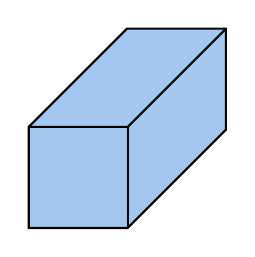
\begin{tikzpicture}[x=0.75pt,y=0.75pt,yscale=-1,xscale=1]
		%uncomment if require: \path (0,300); %set diagram left start at 0, and has height of 300
		
		%Shape: Cube [id:dp9961265448984828] 
		\draw  [fill={rgb, 255:red, 74; green, 144; blue, 226 }  ,fill opacity=0.5 ] (69.33,120.76) -- (116.63,73.47) -- (164.33,73.47) -- (164.33,122.17) -- (117.04,169.47) -- (69.33,169.47) -- cycle ; \draw   (164.33,73.47) -- (117.04,120.76) -- (69.33,120.76) ; \draw   (117.04,120.76) -- (117.04,169.47) ;
		
		
		
		
	\end{tikzpicture}
	
	\caption{\label{fig:tA2}A pictorial demonstration of $\tA\in \Lambda^2(U)\otimes V$.}
\end{figure}

First, following \cite{TI1}, we construct $\tilde\tA\in (U\oplus V)\otimes (U\oplus V)\otimes (U\oplus V)^*$, by putting $\tA$ in the appropriate block, shown in Figure~\ref{fig:tA2_alg}.


\begin{figure}[!htbp]
	
	\centering
	
	
	\tikzset{every picture/.style={line width=0.75pt}} %set default line width to 0.75pt        
	
	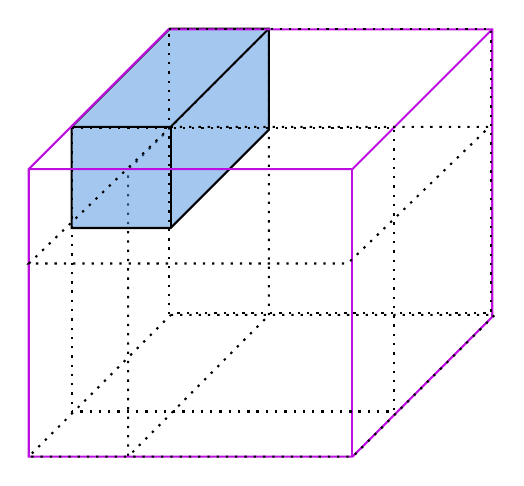
\begin{tikzpicture}[x=0.75pt,y=0.75pt,yscale=-1,xscale=1]
		%uncomment if require: \path (0,300); %set diagram left start at 0, and has height of 300
		
		%Shape: Parallelogram [id:dp2985363659610176] 
		\draw  [dash pattern={on 0.84pt off 2.51pt}] (365,177.2) -- (365,39.16) -- (297.19,107.32) -- (297.19,245.36) -- cycle ;
		%Shape: Cube [id:dp5128329714294058] 
		\draw  [fill={rgb, 255:red, 74; green, 144; blue, 226 }  ,fill opacity=0.5 ] (270,86.46) -- (317.3,39.16) -- (365,39.16) -- (365,87.87) -- (317.7,135.16) -- (270,135.16) -- cycle ; \draw   (365,39.16) -- (317.7,86.46) -- (270,86.46) ; \draw   (317.7,86.46) -- (317.7,135.16) ;
		%Shape: Cube [id:dp18352113751233556] 
		\draw  [color={rgb, 255:red, 189; green, 16; blue, 224 }  ,draw opacity=1 ] (249.33,106.83) -- (316.72,39.44) -- (472.64,39.44) -- (472.64,177.98) -- (405.25,245.36) -- (249.33,245.36) -- cycle ; \draw  [color={rgb, 255:red, 189; green, 16; blue, 224 }  ,draw opacity=1 ] (472.64,39.44) -- (405.25,106.83) -- (249.33,106.83) ; \draw  [color={rgb, 255:red, 189; green, 16; blue, 224 }  ,draw opacity=1 ] (405.25,106.83) -- (405.25,245.36) ;
		%Shape: Rectangle [id:dp3570799785010865] 
		\draw  [dash pattern={on 0.84pt off 2.51pt}] (270,86.96) -- (425.44,86.96) -- (425.44,223.6) -- (270,223.6) -- cycle ;
		%Shape: Parallelogram [id:dp5399948357072122] 
		\draw  [dash pattern={on 0.84pt off 2.51pt}] (317.7,86.46) -- (471.3,86.46) -- (403.03,152.29) -- (249.43,152.29) -- cycle ;
		%Shape: Rectangle [id:dp48572655629770445] 
		\draw  [dash pattern={on 0.84pt off 2.51pt}] (316.72,39.44) -- (472.16,39.44) -- (472.16,176.08) -- (316.72,176.08) -- cycle ;
		%Shape: Rectangle [id:dp46030026846674255] 
		\draw  [dash pattern={on 0.84pt off 2.51pt}] (317.8,177.04) -- (473.83,177.04) -- (405.37,245.36) -- (249.33,245.36) -- cycle ;
		
		
		
		
	\end{tikzpicture}
	
\caption{\label{fig:tA2_alg}A pictorial demonstration of $\tilde\tA\in (U\oplus V)\otimes (U\oplus V)\otimes (U\oplus V)^*$.}
\end{figure}

To show that $\tA\cong \tB$ if and only if $\tilde\tA\cong\tilde\tB$ as in \cite{TI1}, non-degeneracy along $V$ is required. To avoid this, we add two FGS gadgets with certain twists. First, we construct FGS gadgets $\tG_{2(\ell+m+1), \ell}$ and $\tG_{4(\ell+m+1), m}$. We then construct $\tG'_{2(\ell+m+1), \ell}$, a $2(\ell+m+1)\cdot (\ell+1)\times 2(\ell+m+1)\cdot (\ell+1)\times \ell$ tensor, by putting  $\tG_{2(\ell+m+1), \ell}$ to the left-lower subtensor, and zero elsewhere. That is, $\tG'_{2(\ell+m+1), \ell}=\begin{bmatrix}
	0 & 0 \\
	\tG_{2(\ell+m+1), \ell} & 0 
\end{bmatrix}$. Similarly construct $\tG'_{4(\ell+m+1), m}=\begin{bmatrix}
0 & 0 \\
\tG_{4(\ell+m+1), m} & 0 
\end{bmatrix}$. Now install $\tG'_{2(\ell+m+1), \ell}$ and $\tG'_{4(\ell+m+1), m}$ to $\tilde\tA$ as in Figure~\ref{fig:tA2_alg-new}. 



\begin{figure}[!htbp]
	
	\centering
	
	
	
	
	
	\tikzset{every picture/.style={line width=0.75pt}} %set default line width to 0.75pt        
	
	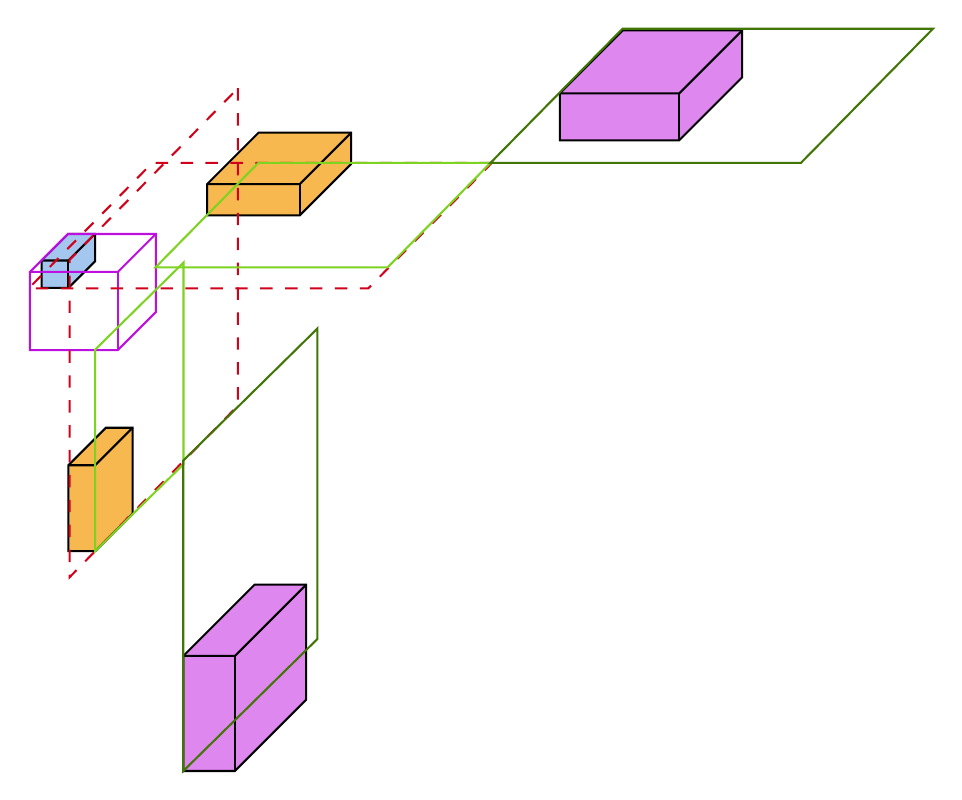
\begin{tikzpicture}[x=0.75pt,y=0.75pt,yscale=-0.7,xscale=0.7]
		%uncomment if require: \path (0,641); %set diagram left start at 0, and has height of 641
		
		%Shape: Cube [id:dp6828276662728947] 
		\draw  [fill={rgb, 255:red, 74; green, 144; blue, 226 }  ,fill opacity=0.5 ] (66.11,281.92) -- (84.47,263.56) -- (102.98,263.56) -- (102.98,282.46) -- (84.63,300.82) -- (66.11,300.82) -- cycle ; \draw   (102.98,263.56) -- (84.63,281.92) -- (66.11,281.92) ; \draw   (84.63,281.92) -- (84.63,300.82) ;
		%Shape: Cube [id:dp9963685009748868] 
		\draw  [color={rgb, 255:red, 189; green, 16; blue, 224 }  ,draw opacity=1 ] (58.09,289.82) -- (84.25,263.67) -- (144.76,263.67) -- (144.76,317.44) -- (118.61,343.59) -- (58.09,343.59) -- cycle ; \draw  [color={rgb, 255:red, 189; green, 16; blue, 224 }  ,draw opacity=1 ] (144.76,263.67) -- (118.61,289.82) -- (58.09,289.82) ; \draw  [color={rgb, 255:red, 189; green, 16; blue, 224 }  ,draw opacity=1 ] (118.61,289.82) -- (118.61,343.59) ;
		%Shape: Cube [id:dp09499126868837227] 
		\draw  [fill={rgb, 255:red, 245; green, 166; blue, 35 }  ,fill opacity=0.8 ] (180.08,229.37) -- (215.53,193.92) -- (279.22,193.92) -- (279.22,215.45) -- (243.77,250.91) -- (180.08,250.91) -- cycle ; \draw   (279.22,193.92) -- (243.77,229.37) -- (180.08,229.37) ; \draw   (243.77,229.37) -- (243.77,250.91) ;
		%Shape: Cube [id:dp8178179216265842] 
		\draw  [fill={rgb, 255:red, 245; green, 166; blue, 35 }  ,fill opacity=0.8 ] (84.61,422.88) -- (110.46,397.04) -- (128.83,397.04) -- (128.83,456.18) -- (102.98,482.02) -- (84.61,482.02) -- cycle ; \draw   (128.83,397.04) -- (102.98,422.88) -- (84.61,422.88) ; \draw   (102.98,422.88) -- (102.98,482.02) ;
		%Shape: Cube [id:dp7491419675661859] 
		\draw  [fill={rgb, 255:red, 189; green, 16; blue, 224 }  ,fill opacity=0.5 ] (422.88,166.87) -- (466.19,123.56) -- (548.32,123.56) -- (548.32,155.89) -- (505.01,199.2) -- (422.88,199.2) -- cycle ; \draw   (548.32,123.56) -- (505.01,166.87) -- (422.88,166.87) ; \draw   (505.01,166.87) -- (505.01,199.2) ;
		%Shape: Rectangle [id:dp6917141582188386] 
		\draw  [color={rgb, 255:red, 208; green, 2; blue, 27 }  ,draw opacity=1 ][dash pattern={on 4.5pt off 4.5pt}] (201.28,163.36) -- (201.28,381.82) -- (85.44,499.9) -- (85.44,281.44) -- cycle ;
		%Shape: Rectangle [id:dp6604630536311706] 
		\draw  [color={rgb, 255:red, 208; green, 2; blue, 27 }  ,draw opacity=1 ][dash pattern={on 4.5pt off 4.5pt}] (376.08,214.72) -- (142.33,214.72) -- (57.28,301.12) -- (291.03,301.12) -- cycle ;
		%Shape: Cube [id:dp0022101522879205415] 
		\draw  [fill={rgb, 255:red, 189; green, 16; blue, 224 }  ,fill opacity=0.5 ] (163.67,554.11) -- (212.77,505.01) -- (248.26,505.01) -- (248.26,584.21) -- (199.16,633.31) -- (163.67,633.31) -- cycle ; \draw   (248.26,505.01) -- (199.16,554.11) -- (163.67,554.11) ; \draw   (199.16,554.11) -- (199.16,633.31) ;
		%Shape: Rectangle [id:dp9633186630913892] 
		\draw  [color={rgb, 255:red, 126; green, 211; blue, 33 }  ,draw opacity=1 ] (375.12,214.72) -- (215.36,214.72) -- (144.48,286.72) -- (304.24,286.72) -- cycle ;
		%Shape: Rectangle [id:dp3938621435779259] 
		\draw  [color={rgb, 255:red, 65; green, 117; blue, 5 }  ,draw opacity=1 ] (679.68,122.4) -- (466,122.4) -- (375.12,214.72) -- (588.8,214.72) -- cycle ;
		%Shape: Rectangle [id:dp8054488160306934] 
		\draw  [color={rgb, 255:red, 126; green, 211; blue, 33 }  ,draw opacity=1 ] (163.84,283.36) -- (163.84,422.11) -- (102.98,482.02) -- (102.98,343.27) -- cycle ;
		%Shape: Rectangle [id:dp9870566466708992] 
		\draw  [color={rgb, 255:red, 65; green, 117; blue, 5 }  ,draw opacity=1 ] (255.99,328.75) -- (255.99,542.43) -- (163.67,633.31) -- (163.67,419.63) -- cycle ;
		
		
		
		
	\end{tikzpicture}
	
	
	
	
	
\caption{\label{fig:tA2_alg-new}A pictorial demonstration of $\bar\tA\in U'\otimes U'\otimes U'^*$. The orange and purple regions indicate the positions of $\tG_{2(\ell+m+1), \ell}$ and $\tG_{4(\ell+m+1), m}$, respectively.}
\end{figure}

Let the resulting tensor be $\bar\tA$. Let $U'=\rng^{\ell+m+2(\ell+m+1)\cdot(\ell+1)+4(\ell+m+1)\cdot(m+1)}$. We claim that $\tA, \tB\in \Lambda^2(U)\otimes V^*$ are isomorphic if and only if $\bar\tA$ and $\bar\tB$ are isomorphic. The only if direction is straightforward by Fact~\ref{fact:FGS-tensor}. For the if direction, let $P\in \GL(U')$ be an isomorphism from $\bar\tA$ to $\bar\tB$. Because of rank considerations, we see that $P=\begin{bmatrix}
	P_{11} & 0 & 0 \\
	0 & P_{22} & 0 \\
	P_{31} & P_{32} & P_{33}
\end{bmatrix}$ where $P_{11}$ is of size $\ell\times \ell$, and $P_{22}$ is of size $m\times m$. So $P_{11}$ and $P_{22}$ are invertible. By examining the $(1, 1, 2)$-position blocks of $P^t\bar\tA P$ and $\bar\tB^P$, we see that $(P_{11}, P_{22})$ form an isomorphism from $\tA$ to $\tB$. 

Finally, we note that a Lie algebra with structural constants in the form of Figure~\ref{fig:tA2_alg-new} satisfies that for any $u, v, w$, $[u, [v, w]]=0$. That is, this is a nilpotent class-$2$ Lie algebra. This concludes the proof.
\end{proof}

\subsubsection{Proof of Corollary~\ref{cor:TIZ-complete}}

The matrix space conjugacy problem corresponds to the orbit problem for $U\otimes U^*\otimes V$. The algebra isomorphism problem corresponds to the orbit problem for $U\otimes U\otimes U^*$. The trilinear form isomorphism problem corresponds to the orbit problem for $U\otimes U\otimes U$. For the Calabi--Yau threefold classification problem, clearly it generalises the trilinear form isomorphism problem. We then reduce it to symmetric trilinear form isomorphism, so to show that it is $\ThreeFTI_\Z$-complete. 

Recall that the Calabi--Yau threefold isomorphism problem considers a pair of a symmetric trilinear form $\phi:\Z^n\times\Z^n\times\dots\times \Z^n\to \N$ and a linear form $f:\Z^n\to \N$. We construct a symmetric trilinear form $\tilde\phi:\Z^{n+1}\times\Z^{n+1}\times\Z^{n+1}$ as follows. First, extend $f:\Z^n\to \N$ to $\tilde f:\Z^{n+1}\to\N$ by $\tilde f(\stdb_i)=f(\stdb_i)$ for $i\in[n]$, and $f(\stdb_{n+1})=0$. We then construct $\tilde\phi:\Z^{n+1}\times\Z^{n+1}\times\Z^{n+1}$ such that (1) when restricting to $\Z^n$ spanned by the first $n$ coordinates, $\tilde\phi|_{\Z_n}=\phi$, (2) the linear form obtained by restricting the first two coordinates to $\stdb_{n+1}$, that is $\tilde\phi(\stdb_{n+1}, \stdb_{n+1}, v)$ for $v\in \Z^{n+1}$, is $\tilde f$, and (3) extend to other unattended entries by symmetry. 

For another pair of $\psi:\Z^n\times\Z^n\times\dots\times \Z^n\to \N$ and $g:\Z^n\to \N$, we apply the above procedure to get $\tilde\psi$. It is easy to see that $(\phi, f)$ and $(\psi, g)$ are isomorphic under $\GL(n, \Z)$ implies that $\tilde\phi$ and $\tilde\psi$ are isomorphic. For the converse direction, we need to ensure that an isomorphism from $\tilde\phi$ to $\tilde\psi$ which is in $\GL(n+1, \Z)$ does not mix up the first $n$ coordinates and the last coordinate. This can be done by adding the same gadget as in the proof of Theorem~\ref{thm:Lambda3U}. Therefore, we blow-up the dimensions even further, but they are polynomially bounded so that would be fine. This concludes the proof of Corollary~\ref{cor:TIZ-complete}.


\subsection{General modules over finite local principal ideal rings}\label{subsec:five-action-PIR}

Over finite local principal ideal rings (PIRs), a suitable notion of degeneracy can be defined, and a reduction from degenerate to non-degenerate cases can be achieved via the GQ gadget. In this part, we present the main ingredients for adapting the GQ gadget to this seting. 

\paragraph{Some key points for adapting GQ gadgets.} The GQ gadget was reviewed in Section~\ref{sec:GQ}. There are three identity matrices in the added slices (cf. $\tilde C_{m+2}$ in Equation~\ref{eq:GQ}): 
\begin{enumerate}
	\item One identity matrix ($\idmat_{2(n+6)}$ in $\tilde C_{m+2}$) responsible for large enough rank so this slice does not add to others,
	\item A second identity matrix ($\idmat_{n}$ in $\tilde C_{m+2}$) responsible for clearing out those parts added to it, 
	\item A third identity matrix ($\idmat_{2}$ in $\tilde C_{m+2}$) for ensuring the transformation matrices to have a zero-block, so it is in a suitable block diagonal structure.
\end{enumerate}
Once the transformation matrices are put in a block diagonal structure, a non-degeneracy condition is used to ensure that the original tensors get transformed by invertible matrices.

All these properties need to be taken care of for $\Z/p^e\Z$ modules, but they are achievable via the following ingredients. Instead of repeating the proofs from \cite{TI4}, we shall only indicate the key points for achieving Theorem~\ref{thm:ptoe-equivalence} as follows. 

Here we give a brief summary. 
\begin{itemize}
	\item First, we need the diagonal-full property, satisfied by local rings as shown in Section~\ref{subsec:diagonal-full}.
	\item In Section~\ref{subsec:nondeg}, we introduce the non-degeneracy definitions suitable for our purpose. We need two conditions for rings: (1) non-zero non-units are zero-divisors, satisfied by finite rings, and (2) the existence of Smith Normal Forms, satisfied by PIRs.
	\item In Section~\ref{subsec:invertible}, we present a result which suggests that, over $\Z/p^e\Z$, if the transformation matrix preserves the gadget slices, then its diagonal blocks are invertible, despite that it may not be in the strict block upper-triangular structure.
	\item After these, we indicate the differences of the construction needed compared with \cite{TI4} in Remark~\ref{rem:TI4}.
\end{itemize}


\subsubsection{The issue of non-degeneracy}\label{subsec:nondeg}

\paragraph{Non-degeneracy of bilinear forms.}
Let $\rng$ be a commutative ring. 
Let $U$ and $V$ be two modules over $\rng$, and let $f:U\times V\to \rng$ be a bilinear form. For $u\in U$, $f_u:V\to \rng$ is an $\rng$-linear form sending $v\in V$ to $f_u(v)=f(u, v)$. Define $\ker_U(f)=\{u\in U\mid f_u=0\}$. We say that $f$ is \emph{degenerate} along $U$, if $\ker_U(f)$ is non-trivial.
\begin{observation}\label{obs:unit-zd}
	Let $\rng$ be a commutative ring such that every non-unit is a zero-divisor. Let $U$ and $V$ be two modules over $\rng$, and let $f, g:U\times V\to \rng$ be bilinear forms. Suppose there exists $L\in\M(m, \rng)$ such that $f(L(u), v)=g(u, v)$. If $g$ is left non-degenerate, then $L\in\GL(m, \rng)$. 
\end{observation}
\begin{proof}
	For the sake of contradiction, suppose $L\not\in\GL(m, \rng)$. So $\det(L)$ is not a unit, so it is a zero-divisor or 0, which implies that there exists a non-zero $u'\in U$, $Lu'=0$. By $f(L(u), v)=g(u, v)$, this implies that $g(u, v)=f(0, v)=0$, contradicting to that $g$ is non-degenerate.
\end{proof}
%\begin{observation}
%	Let $\rng$ be a commutative ring such that every non-unit is a zero-divisor. Let $A, B\in\M(m\times n, \rng)$. Suppose there exists $L\in\M(m, \rng)$ such that $LA=B$. If $B$ is non-degenerate, then $L\in\GL(m, \rng)$. 
%\end{observation}
%\begin{proof}
%	For the sake of contradiction, suppose $L\not\in\GL(m, \rng)$. So $\det(L)$ is not a unit, so it is a zero-divisor or 0, which implies that there exists a non-zero $v\in \rng^m$, $vL=0$. By $LA=B$, this implies that $vB=0$, contradicting to that $B$ is non-degenerate.
%\end{proof}
Note that a finite ring satisfies that every non-zero element is either a unit or a zero-divisor. Also note that in $\Z$ every non-zero non-unit is a non-zero-divisor, so Observation~\ref{obs:unit-zd} would not be useful in that setting.

\paragraph{Reducing to non-degenerate for bilinear forms over PIRs.}
%\ynote{Where is the local condition used in the part? More specifically, what would go wrong if we work with $\Z/6\Z$?}
Now set $\rng$ to be a PIR with the maximal ideal $\m$ with nilpotency index $e$. Let $U$ and $V$ be modules over $\rng$. 

%Suppose $U\cong \bigoplus_{i\in[s]} \rng/\m^{a_i}$ with $1 \leq a_i \leq e$, and $V\cong \bigoplus_{i\in[t]} \rng/\m^{b_i}$ with $1\leq b_i\leq e$. Let $f:U\times V\to \rng$ be a bilinear form and assume that $K:=\lker(f)$ is non-trivial. Then $f$ can be represented as an $s\times t$ matrix $A_f$ over $\rng$.

Let $f:U\times V\to \rng$ be a bilinear form and assume that $K:=\ker_U(f)$ is non-trivial. 
By Smith Normal Form, there is a basis $\stdb_1,\dotsc,\stdb_s$ for $U$, together with an integer $r\in[s]$, and exponents $0 \leq k_1 \leq k_2 \leq \dots k_r$  such that $t^{k_1} \stdb_1, t^{k_2} \stdb_2, \dotsc, t^{k_r} \stdb_r$ form a basis for $K$. By our assumption, we can compute this SNF in polynomial time, which includes the elements $\stdb_i$ and the exponents $k_i$.

Suppose under this basis, $U\cong \bigoplus_{i\in[s]} \rng/\m^{a_i}$. Suppose that $V\cong \bigoplus_{i\in[t]} \rng/\m^{b_i}$ with $1\leq b_i\leq e$. Then $f$ can be represented as an $s\times t$ matrix $A_f$ over $\rng$, with the first $r$ rows of $A_f$ corresponding to $\lker(f)$ after multiplying suitable powers of $t$. 

As $t^{k_i}\stdb_i\in \lker(f)$ for $i\in[k]$, it follows that the $i$th row of $A_f$ is divisible by $t^{a_i-k_i}$. Set $\tilde U=(\oplus_{i\in[r]}\rng/\langle t^{k_i}\rangle)\oplus (\oplus_{r+1\leq i\leq s}\rng/\langle t^{a_i}\rangle)$, with $k_i=0$ understood as removing that coordinate. Construct the following matrix $\tilde A_f$: starting from $A$, for $i\in[r]$, if $k_i=0$, then delete the $i$th row of $A$. If $k_i>0$, then mod out $t^{e-k_i}$ on the $i$th row of $A_f$. Then $\tilde A_f$ represents a bilinear form $\tilde f:\tilde U\times V\to \rng$. It can be verified easily that $\tilde f$ is non-degenerate. 

Furthermore, let $f, g:U\times V\to \rng$ be two bilinear forms, and let $\tilde f, \tilde g:\tilde U\times V\to\rng$ be the resulting bilinear forms from the above procedure. It can also be verified easily that $f$ and $g$ are left-equivalent (under $\GL(U)$) if and only if $\tilde f$ and $\tilde g$ are left-equivalent (under $\GL(\tilde U)$). %\ynote{Do we need more details here?}


\paragraph{Non-degeneracy for trilinear forms and bilinear maps, and reductions to non-degenerate case.} Let $\rng$ be a commutative ring. Let $U, V, W$ be three modules over $\rng$, and $f:U\times V\times W\to\rng$ be a trilinear form. We say that $f$ is non-degenerate along $U$, if $f$ viewed as a bilinear form $U\times (V\otimes W)\to \rng$ is non-degenerate along $U$. Non-degeneracy along $V$ or $W$ is defined similarly.

Given a bilinear map $f:U\times U\to V$, and $u\in U$, let $f_u:U\to V$ be the $\rng$-linear map from $U$ to $V$ defined as $f_u(u')=f(u, u')$. Let $f':U\times U\times V^*\to \rng$ be the trilinear form associated with $f$. We can then define left, right, and image non-degeneracies for $f$ by non-degeneracies of $f'$ along the first $U$, the second $U$, and $V^*$. 

%Let the left kernel of $f$ be $\lker(f):=\{u\in U\mid f_u=0\}$. We say that $f$ is left non-degenerate, if $\lker(f)=0$. The right non-degeneracy is defined analogously. Note that if $f$ is symmetric or alternating, then left and right non-degeneracies coincide. We say that $f$ isnon-degenerate along $V$, if the annihilator of the image $\Ann(f)=\{h\in V^*\mid h(f(U, U))=0\}$ is zero. In other words, the 
%image non-degenerate, if $\im(f)=\{f(u, u')\mid u, u'\in U\}$ is equal to $V$. 

%\paragraph{Reducing to non-degenerate for trilinear forms and bilinear maps over local PIRs.} 

The reduction to non-degeneracy in the bilinear form setting applies to trilinear forms and bilinear maps. This is evident because non-degeneracy is defined in accordance with the bilinear form case. 

\subsubsection{The invertible diagonal lemma}\label{subsec:invertible}

\begin{lemma}[{cf. \cite[Lemma~2.2 and Lemma~5.2]{TI4}}]\label{lem:invertible}
	Suppose $P \Gamma P^t = \Gamma$, where
	\[
	\Gamma = \begin{bmatrix}
		A & 0 & 0 \\ 
		0 & p^{e-1} J_r & 0 \\
		0 & 0 & 0 
	\end{bmatrix}
	\]
	where $J_r = \begin{bmatrix} 0 & I_r \\ -I_r & 0 \end{bmatrix}$, and $r > 2n$, and $A$ is some invertible $n \times n$ (alternating) matrix. If we write
	\[
	P = \begin{bmatrix} 
		P_{11} & P_{12} & P_{13} \\
		P_{21} & P_{22} & P_{23} \\
		P_{31} & P_{32} & P_{33}
	\end{bmatrix}
	\]
	with block sizes commensurate with the blocks of $\Gamma$ above, then $P \pmod{p}$ is block-upper-triangular, $P_{11}, P_{22}, P_{33}$ are invertible, and there is an invertible matrix $Q_{11}$ (such that $Q_{11} \equiv P_{11}^{-1} \pmod{p}$) such that $P_{11} A Q_{11}^{-t} = A$.
\end{lemma}

\begin{proof}
	For simplicity of notation, let $Q = P^{-1}$. Then our equation becomes $P \Gamma Q^{-T} = \Gamma$, or equivalently $P \Gamma = \Gamma Q^t$. Write $Q$ as a $4 \times 4$ matrix similar to $P$. Then we have the following equation
	\[
	\begin{bmatrix} 
		P_{11} & P_{12} & P_{13} \\
		P_{21} & P_{22} & P_{23} \\
		P_{31} & P_{32} & P_{33} 
	\end{bmatrix}
	\begin{bmatrix}
		A & 0 & 0 \\
		0 &p^{e-1} J_r & 0 \\
		0 & 0 & 0 
	\end{bmatrix}
	= 
	\begin{bmatrix}
		A & 0 & 0 \\
		0 &p^{e-1} J_r & 0 \\
		0 & 0 & 0 
	\end{bmatrix}
	\begin{bmatrix} 
		Q_{11}^t & Q_{21}^t & Q_{31}^t \\
		Q_{12}^t & Q_{22}^t & Q_{32}^t \\
		Q_{13}^t & Q_{23}^t & Q_{33}^t \\
	\end{bmatrix}
	\]
	Multiplying out, this gives us
	\[
	\begin{bmatrix} 
		P_{11} A & p^{e-1}P_{12} & 0 \\
		P_{21} A & p^{e-1}P_{22} & 0\\
		P_{31} A & p^{e-1}P_{32} & 0
	\end{bmatrix}
	= 
	\begin{bmatrix} 
		A Q_{11}^t & A Q_{21}^t & A Q_{31}^t \\
		p^{e-1}Q_{12}^t & p^{e-1}Q_{22}^t & p^{e-1}Q_{32}^t \\
		0 & 0 & 0
	\end{bmatrix}
	\]
	From these, we immediately get $P_{31} A = 0$ and since $A$ is invertible, we get $P_{31} = 0$. We also get that $p$ divides $P_{32}$, since $p^{e-1} P_{32} = 0$, and we are working modulo $p^e$. We also get that $P_{21} A = p^{e-1} Q_{21}^t$, so $P_{21} A$ is divisible by $p^{e-1}$. Again, since $A$ is invertible, we find $P_{21} = p^{e-1} Q_{12}^t A^{-1}$, so $P_{21}$ is divisible by $p^{e-1}$. Thus $P$ has the form
	\[
	P = \begin{bmatrix}
		P_{11} & * & * \\
		p^{e-1} * & P_{22} & * \\
		0 & p * & P_{33}
	\end{bmatrix}
	\]
	where the $*$'s may be arbitrary. However, a matrix over $\Z/p^e \Z$ is invertible iff it is invertible modulo $p$ \cite{Ranum, HillarRhea}. Since $P$ is invertible by assumption and $P\pmod{p}$ is block-upper-triangular, we have that $P_{ii} \pmod{p}$ is invertible for $i=1,2,3$, and hence $P_{ii}$ itself (not modulo $p$) is invertible for $i=1,2,3$. 
	
	From the (1,1) entry above, note that we have $P_{11} A = A Q_{11}^t$. It remains to show that $Q_{11}$ is invertible, for then we will have $P_{11} A Q_{11}^{-t} = A$, as claimed.
	
	Similar to $P$, we find that $Q_{31} = 0$, $Q_{32}$ must be divisible by $p$, and $Q_{21}$ must be divisible by $p^{e-1}$. Thus $Q$ has the form
	\[
	Q = \begin{bmatrix}
		Q_{11} & * & * \\
		p^{e-1}* & Q_{22} & * \\
		0 & p* & Q_{33}
	\end{bmatrix}.
	\]
	As with $P$, we find that each $Q_{ii}$ is invertible modulo $p$, hence invertible, thus completing the proof.
\end{proof}

\begin{remark}\label{rem:TI4}
	Given the above preparations, in order to accommodate the gadgets of \cite{TI4}, we expand the rows to accommodate two copies of the rows, plus enough copies of $\Z / p \Z$ (n.b.: $p$, not $p^e$!) to make room for the $p^{e-1} J_r$ gadget. This results in the complex parameter increasing by only a polynomial factor, and then with the preceding lemma in hand, as well as the use of inner rank instead of rank, the results of \cite{TI4} go through. 
\end{remark}
%
%\paragraph{Equivalence of five actions over finite local PIRs.} With the above preparations, we can state our result. First recall that for a local ring $\rng$, the rank of an $\rng$-module $M$ is defined to be the size of a minimal generating set, which is uniquely determined by Nakayama's lemma.
%
%Let $\rng$ be a finite local PIR. Let $U$, $V$, $W$ be $\rng$-modules. The \emph{length} of $\tA\in U\otimes V\otimes W$ is defined to be the sum of ranks of $U$, $V$, and $W$. Note that $\rng$ satisfies the diagonal-full condition as explained in Section~\ref{subsec:diagonal-full}.
%\begin{theorem}
%	Let $\rng$ be a finite local PIR. Let $U$, $V$, $W$ be $\rng$-modules. The orbit problems for the following actions are polynomial-time equivalent. 
%	\begin{enumerate}
%		\item $\GL(U)\times\GL(V)\times\GL(W)$ on $U\otimes V\otimes W$. 
%		\item $\GL(U)\times \GL(V)$ on $\S^2(U)\otimes V$ and $\Lambda^2(U)\otimes V$. 
%		\item $\GL(U)\times \GL(V)$ on $U\otimes U^*\otimes V$. 
%		\item $\GL(U)$ on $\S^3(U)$ and $\Lambda^3(U)$. 
%		\item $\GL(U)$ on $U\otimes U\otimes U^*$.
%	\end{enumerate}
%	In particular, the reduction from action $i$ to action $j$ satisfies that: it is a polynomial fnction $f$ that takes $\tA$ and $\tB$ for one action, and produces $f(\tA)$ and $f(\tB)$ for the other action, such that the lengths of $f(\tA)$ and $f(\tB)$ are linear in the lengths of $\tA$ and $\tB$.
%\end{theorem}
%\ynote{A proof sketch needs to be here. Due to time limitation it would be probably just something like ``plugging the above to TI4''.}
